\documentclass[hidelinks,a4paper,12pt, nofootinbib]{article}
\usepackage[width=15.5cm, left=3cm, top=2.5cm, right=2cm, left=2cm, height= 24.5cm]{geometry}
\usepackage[spanish, es-tabla]{babel} %es-tabla es para que ponga Tabla en vez de Cuadro en el caption
\usepackage[utf8]{inputenc}
\usepackage[T1]{fontenc}
\usepackage{xspace}
\usepackage{xargs}
\usepackage{fancyhdr}
\usepackage{lastpage}
\usepackage{caratula}
\usepackage[bottom]{footmisc}
\usepackage{amssymb}
\usepackage{algorithm}
\usepackage[noend]{algpseudocode}
\usepackage{array}
\usepackage{xcolor,colortbl}
\usepackage{amsthm}

\usepackage{pgf}
\usepackage{tikz}
\usetikzlibrary{arrows,automata}

\usepackage{graphicx}
\usepackage{sidecap}
\usepackage{amsmath}
\usepackage{wrapfig}
\usepackage{caption}

\usepackage{hyperref}
\hypersetup{
  colorlinks   = true, %Colours links instead of ugly boxes
  urlcolor     = blue, %Colour for external hyperlinks
  linkcolor    = blue, %Colour of internal links
  citecolor   = red %Colour of citations
}

\usepackage{comment}

\usepackage[
  backend=bibtex,
  style=alphabetic
]{biblatex}
\addbibresource{bibliografia.bib}


\captionsetup[table]{labelsep=space}


\setlength{\parindent}{4em}
\setlength{\parskip}{0.5em}

%Defino colores para las tablas
\definecolor{LightCyan}{rgb}{0.77,0.9,0.9}
\definecolor{Gray}{gray}{0.8}


%%fancyhdr
\pagestyle{fancy}
\thispagestyle{fancy}
\addtolength{\headheight}{1pt}
\lhead{Aalgoritmos y Estructuras de Datos III: TP1}
\rhead{$1º$ cuatrimestre de 2016}
\cfoot{\thepage\ / \pageref{LastPage}}
\renewcommand{\footrulewidth}{0.4pt}

%%caratula
\materia{Algoritmos y Estructuras de Datos III}
\titulo{Trabajo Práctico Número 1}
%\subtitulo{}
%\grupo{Grupo 12}
\integrante{Ciruelos Rodríguez, Gonzalo}{063/14}{gonzalo.ciruelos@gmail.com}
\integrante{Costa, Manuel José Joaquín}{035/14}{manucos94@gmail.com}
\integrante{Gatti, Mathias Nicolás}{477/14}{mathigatti@gmail.com}
\integrante{Maddonni, Axel}{200/14}{axel.maddonni@gmail.com}

\fecha{8 de Abril de 2016}

\usepackage{etoolbox}
\AtBeginEnvironment{tikzpicture}{\shorthandoff{>}\shorthandoff{<}}{}{}

\begin{document}
\maketitle

\tableofcontents
\newpage

\section{Kaio Ken}

\subsection{Explicación formal del problema}

Para entender mejor el problema, lo especificaremos usando términos matemáticos. Se tiene un conjunto de $n$ elementos que representan a los guerreros. 
\[G = \{g_1,...,g_n\}\]

Definiremos una \emph{partición} (\emph{pelea} en el enunciado) como un par de dos conjuntos disjuntos no vacíos de elementos $A$ y $B$ (donde cada uno representa cada bando en una pelea). En cada partición, la unión de dichos conjuntos es el conjunto total de los elementos (es decir, todos los guerreros participan de todas las peleas):
\[ P = (A, B)\]
donde $A$, $B$ son conjuntos de elementos y  \[A \ \dot{\cup}\ B = G.\]

Notaremos $P_A$ al conjunto $A$ de elementos que representa al primer elemento de la partición $P$, y $P_B$ al del otro. Además, para todo elemento $g_k$, notaremos $B_P(g_k)$ (bando, en los t\'erminos del enunciado) al conjunto de la partición $P$ al que $g_k$ pertenece. O sea que los valores que puede tomar $B_P(g_k)$ son $P_A$ o $P_B$. 

Dada una cantidad de elementos $n$, se pide encontrar el conjunto de tamaño mínimo de particiones de modo que para todo par de elementos $(g_i, g_j)$, exista partición $P$ tal que $B_P(g_i) \neq B_P(g_j)$. Veamos algunos ejemplos gráficamente, donde cada cuadrado representa un guerrero, y su color el bando al que pertenece en cada partición:

\begin{figure}[H]
\centering
\begin{minipage}{0.25\textwidth}
  \centering
    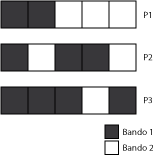
\includegraphics[width=1\textwidth]{img/ejemplos/ej1-1.png}
  \caption*{\footnotesize Posible solución correcta con 3 particiones.}
  \label{fig:ej1-1}
\end{minipage}%
\hspace{0.05\textwidth}
\begin{minipage}{0.25\textwidth}   
  \centering
    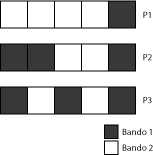
\includegraphics[width=1\textwidth]{img/ejemplos/ej1-2.png} 
  \caption*{\footnotesize Posible solución correcta con 3 particiones.}
  \label{fig:ej1-2}
\end{minipage}%
\hspace{0.05\textwidth}
\begin{minipage}{0.25\textwidth}   
  \centering
    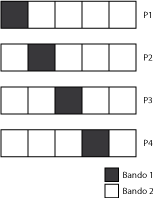
\includegraphics[width=1\textwidth]{img/ejemplos/ej1-3.png} 
  \caption*{\footnotesize Solución incorrecta con 4 particiones.}
  \label{fig:ej1-3}
\end{minipage}%
\caption{Ejemplo con n=5}
\end{figure}

Notar que puede haber más de una solución correcta. El algoritmo propuesto devuelve una de ellas.

\begin{figure}[H]
\centering
\begin{minipage}{0.25\textwidth}
  \centering
    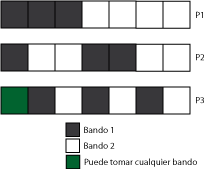
\includegraphics[width=1\textwidth]{img/ejemplos/ej1-4.png}
  \caption*{\footnotesize Posible solución correcta con 3 particiones.}
  \label{fig:ej1-4}
\end{minipage}%
\hspace{0.1\textwidth}
\begin{minipage}{0.25\textwidth}   
  \centering
    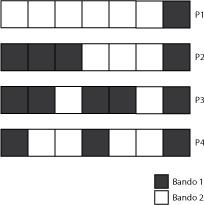
\includegraphics[width=1\textwidth]{img/ejemplos/ej1-5.png} 
  \caption*{\footnotesize Solución incorrecta con 4 particiones.}
  \label{fig:ej1-5}
\end{minipage}%
\caption{Ejemplo con n=7}
\label{fign7}
\end{figure}

\subsection{Explicación de la solución}

Para explicar la solución, mezclaremos el lenguaje del problema original con el lenguaje formal, usando el que creamos que hará más clara la explicación en cada momento.

Para resolver el problema, utilizamos un algoritmo usando la técnica de \textbf{divide and conquer}, es decir, dividimos el problema en subproblemas más pequeños, los resolvemos, y luego combinamos las soluciones para lograr la solución al problema total.

Para entender cómo lo aplicamos para resolver el problema, consideremos la primera partición: $P_1$, cuando todavía no comenzaron los guerreros a pelear.
Para dicha pelea, se eligen guerreros para el bando $P_{1A}$ y para el bando $P_{1B}$, de modo que luego de la pelea, todos los guerreros del bando A hubieron peleado contra los del B y viceversa.
De este modo, a los guerreros del bando A, les faltará solamente pelear entre sí, al igual que los del bando B.

Ahora bien, tenemos dos subproblemas separados: 
\begin{itemize}
\item Por un lado, necesitamos que todos los guerreros de $P_{1A}$ peleen entre sí, en la cantidad mínima de peleas posible.
\item Por otro lado, buscaremos lo mismo para los guerreros de $P_{1B}$.
\end{itemize}

Una vez resueltos estos subproblemas, la manera de combinar las soluciones es simple. Supongamos que para la siguiente pelea, los guerreros de $P_{1A}$ se dividen en dos bandos: $C$ y $D$, y los guerreros de $P_{1B}$ se dividen en los bandos $E$ y $F$. Podemos combinar la solución en una única pelea $P_2$, tomando $P_2$ = $(C \cup E,\ D \cup F)$, de modo que en una misma pelea se logren enfrentar los guerreros de $C$ y $D$, y de $E$ y $F$. De la misma forma procedemos para las siguientes peleas.

Podría pasar que cuando aplicamos el algoritmo para resolver los dos subproblemas, ambas subsoluciones resulten con distinta cantidad de peleas necesarias para resolver uno y otro. En ese caso necesitaremos como mínimo el máximo entre las dos. Los guerreros que ya pelearon contra todos sus contrincantes para dichas peleas, se asignarán a cualquier bando ya que es indistinto.

Repetimos el mecanismo hasta llegar al caso base, correspondiente a cuando queremos hacer que 2 guerreros peleen en la mínima cantidad de peleas necesarias. En  este caso sólo se necesita 1 pelea, un guerrero para cada cada bando. En caso de que la cantidad de guerreros de un conjunto sea impar, llegaremos al caso $n=1$. Este caso proviene de dividir previamente un conjunto de 3 guerreros $g_1, g_2, g_3$ en los bandos $g_1$ y  $g_2, g_3$ respectivamente, de modo que el guerrero que queda solo ($g_1$) ya peleó contra los otros dos, y hubo completado todas las peleas contra los demás guerreros, así que el caso $n$ = 1 está resuelto.

Para dividir en subproblemas, el algoritmo presentado divide al conjunto inicial de guerreros a la mitad, es decir, los subconjuntos generados para cada bando son:
\[A = \{g_1,...,g_{\frac{n}{2}}\}\] 
\[B = \{g_{\frac{n}{2}+1},...,g_n\}\]
y luego aplicamos recursión para aplicar el algoritmo a cada bando. Gráficamente:

\begin{figure}[H]
\centering
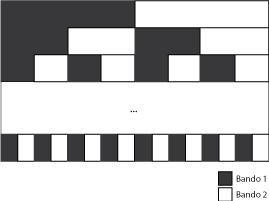
\includegraphics[width=0.50\textwidth]{img/ejemplos/ej1-6.png}
\label{fig:ej1-6}
\caption{Gráfico ilustrativo del algoritmo D\&C propuesto}
\end{figure}

Notar que en caso de que $n$ no sea una potencia de 2, en la última partición aparecerán guerreros que pueden tomar cualquier bando debido a que para ese momento ya pelearon contra todos los demás. Por ejemplo, en la solución al ejemplo con $n=7$ de la figura \ref{fign7} (obtenida por el algoritmo presentado), se encuentra resaltado en la última partición un guerrero al que se le puede asignar cualquier bando.

\subsubsection{Pseudocódigo}
Veamos el pseudocódigo:

\newpage

\begin{algorithm}
\begin{algorithmic}
\caption{Esbozo del algoritmo de KaioKen}
  \Procedure{generarpeleas}{int $n$, int $pactual$, int $inicio$}
  \If {$n = 1$}
    \State $matrizpeleas[pactual][inicio] \gets 1$
  \EndIf
  \If {$n = 2$}
    \State $matrizpeleas[pactual][inicio] \gets 1$
    \State $matrizpeleas[pactual][inicio + 1] \gets 2$
  \Else
    \For {$j \in [0,..., n)$}
      \If {$j < \frac{n}{2}$}
        \State $matrizpeleas[pactual][inicio + j] \gets 1$
      \Else 
        \State $matrizpeleas[pactual][inicio + j] \gets 2$
      \EndIf
    \EndFor
    \State $generarpeleas(\frac{n}{2}, pactual+1, inicio)$
    \State $generarpeleas(\frac{n+1}{2}, pactual+1, n/2 + inicio)$
  \EndIf
  \EndProcedure
\end{algorithmic}
\end{algorithm}

Los resultados obtenidos se van guardando en una matriz (utilizando índices pasados por parámetro para saber qué lugar corresponde a cada guerrero), de forma que una vez calculadas todas las peleas, se imprima la matriz que indica el bando (1 o 2) de cada uno en cada una de las peleas. Esta matriz tiene un tamaño fijo de $n$ columnas y $cantpeleas$ filas, donde 
\[ cantpeleas = \lceil \log _2 n \rceil. \]
 es decir, hay una fórmula cerrada para saber la cantidad de peleas que genera nuestro algoritmo, y proviene de dividir en cada paso el $n$ en mitades iguales. Es decir, por ejemplo:
\begin{itemize}
\item Para $n = 4$, $cantpeleas$ = 2.
\item Para $n = 5,...,8$, $cantpeleas$ = 3.
\item Para $n = 9$, $cantpeleas$ = 4.
\item etc...
\end{itemize}
En la siguiente sección demostraremos por qué este algoritmo resuelve el problema de manera óptima.

\subsubsection{Correctitud}

A diferencia del resto de los problemas, en los que probaremos en conjunto correctitud y optimalidad, en este problema optamos por separar las demostraciones para hacerlas más simples para el lector.

\textbf{Proposición.} El algoritmo es correcto.

\textbf{Demostración.}  Por inducción en $n$.

\textit{Caso Base:} $n = 2$. El algoritmo lo resuelve en una sola pelea, donde cada guerrero pertenece a un bando distinto, $\Pi = {(1,2)}$. Nótese que se cumple lo pedido.

\textit{Paso Inductivo}: Supongo que vale HI: $\forall k \in \mathbb{N}, k \leq n$, vale que el algoritmo es correcto para una entrada de tamaño $k$, con $n \geq 2$.

Entonces seguimos los pasos del algoritmo, dividimos los $n$ elementos en 2 mitades, y usamos el algoritmo para resolver esas 2 mitades. Como cada mitad tiene menos elementos que $n$, entonces el algoritmo es correcto por HI, y las peleas generadas hacen que todos peleen contra todos. Ahora bien, además se agrega una pelea en la que se le asigna al primer grupo el bando 1, y al segundo grupo el bando 2.

Entonces, formalmente, tomemos un par de guerreros $(g_i, g_j)$. Si estos guerreros pertenecen a la misma partición que hicimos al principio para llamar recursivamente al algoritmo, entonces seguro pelean por HI, dado que el algoritmo es correcto para instancias menores a $n$. Si pertenecen a distintas particiones, entonces la nueva pelea les asignará bandos distintos, haci\'endolos pelear. Esto completa la demostración.

\subsubsection{Optimalidad}

Demostraremos que el algoritmo propuesto para resolver el problema es correcto y óptimo, es decir, devuelve un conjunto de peleas de tamaño mínimo para que todos los guerreros hayan peleado entre sí. Usaremos \textbf{índucción global en n}:

Sea $p(n)$ = $"$El algoritmo D\&C propuesto resuelve el problema para $n$ guerreros de manera óptima, generando $\lceil \log _2 n \rceil$ peleas$"$. 

\textit{Caso Base:} $p(2)$. El algoritmo lo resuelve en una sola pelea, donde cada guerrero pertenece a un bando distinto, y es la mejor manera de resolverlo dado que no hay otra manera de que peleen entre sí sin generar al menos 1 pelea.

\textit{Paso Inductivo}: Supongo que vale HI: $\forall k \in \mathbb{N}, k \leq n$, vale $p(k)$, con $n \geq 2$.

Quiero ver que vale $p(n+1)$.
Tengo $n+1$ guerreros. Para la primera pelea, tengo que dividir los guerreros en dos bandos $A$ y $B$, de modo que se generan 2 subproblemas de tamaño $|A|$ y $|B|$.

Por HI, dichos subproblemas los puedo resolver óptimamente, generando $\lceil \log _2 k \rceil$ peleas, donde $k$ es la cantidad de guerreros del subproblema. Quiero ver de qué manera conviene dividir el conjunto inicial de guerreros para que la cantidad de peleas total del problema sea la mínima.
Aplicando el algoritmo en cada bando, la $cantpeleas$ total del problema se puede calcular como: 
\[ cantpeleas = 1 + max\{ \lceil \log _2 |A| \rceil , \lceil \log _2 |B| \rceil \}\]
Esta cantidad se minimiza tomando $|A| = |B| = \frac{n+1}{2}$, en caso de que $n+1$ sea par, o $|A| = \frac{n+1}{2}$ y $|B| = \frac{n+1}{2} + 1$ en caso de que sea impar. Entonces, demostramos que aplicando el algoritmo de D\&C para $n+1$ también llegamos a una solución óptima.

Falta ver que, para $n+1$,  $cantpeleas = \lceil \log _2 (n+1) \rceil$.

Si $n+1$ es par, entonces
  \begin{equation}
  \begin{aligned}
  cantpeleas =& 1 + \lceil \log _2 |A| \rceil \\
  cantpeleas =& 1 + \lceil \log _2 \frac{n+1}{2} \rceil \\
  cantpeleas =& 1 + \lceil \log _2 (n+1)  - 1 \rceil \\
  cantpeleas =& 1 + \lceil \log _2 (n+1) \rceil  - 1 \\
  cantpeleas =& \lceil \log _2 (n+1) \rceil \\
  \end{aligned}
  \end{equation}

Que es lo que queríamos probar.

Si $n + 1$ es impar (y por lo tanto, no es potencia de 2), entonces existe $k > 0$ tal que $2^k < n + 1 < 2^{k+1}$.
Además, podemos tomar
  $A = \lceil \frac{n+1}{2} \rceil = \frac{n+2}{2}$ y
  $B = \lfloor \frac{n+1}2 \rfloor = \frac{n}2$.
Ahora bien, calculemos $cantpeleas$,

  \begin{equation}
  \begin{aligned}
  cantpeleas =& 1 + \lceil \log _2 |A| \rceil \\
  cantpeleas =& 1 + \lceil \log _2 \frac{n+2}{2} \rceil \\
  cantpeleas =& 1 + \lceil \log _2 (n+2) \rceil  - 1 \\
  cantpeleas =& \lceil \log _2 (n+2) \rceil \\
  \end{aligned}
  \end{equation}

Ahora bien, notemos que, como dijimos antes, $2^k < n + 1 < 2^{k+1}$. Entonces, $2^k < n + 1 < n + 2 \leq 2^{k+1}$. Por lo tanto, $k < \log_2(n + 1) < \log_2(n + 2) \leq k +1$. Por lo tanto, $\lceil \log _2 (n+1) \rceil = \lceil \log _2 (n+2) \rceil = k + 1$, por lo tanto 
\[cantpeleas = \lceil \log _2 (n+1) \rceil\]

Que es lo que queríamos ver.

Esto completa la demostración de que el algoritmo encuentra una solución óptima.

\subsection{Complejidad del algoritmo}

El análisis de complejidad es simple, es un algoritmo de Divide \& Conquer clásico, que divide siempre el trabajo en 2 y luego fusiona los resultados de los subproblemas en tiempo $O(n)$. Haciendo una analogía, por ejemplo, con el algoritmo de MergeSort, se puede predecir fácilmente que la complejidad será de $O(nlogn)$.

\subsubsection{Esbozo del algoritmo}

Como puede verse en el pseudocódigo, tenemos dos casos base que toman tiempo constante en ser resueltos.

Por otro lado, el tercer caso realiza un trabajo de costo lineal, escribiendo $n$ entradas de la matriz, y luego hace 2 llamadas recursivas, dividiendo el trabajo en 2 mitades iguales (en caso de que $n$ sea impar, la segunda mitad va a tener un elemento más).

\subsubsection{Análisis temporal}
Si quisieramos expresar la cantidad de operaciones que realiza el algoritmo para un input de tamaño $n$, podríamos escribirlo de la siguiente manera:
\[T(1) = 1\]
\[T(2) = 2\]
\[T(n) = n + 2 T \left(\frac{n}{2}\right)\]

Ahora podemos usar el teorema maestro. El teorema maestro se refiere a relaciones de recurrencia de la pinta:

\[T(n) = f(n) + a T\left(\frac{n}{b}\right)\]

Y afirma, entre otras cosas, que si $f(n) \in O(n^c \log^k n)$ donde $c = \log_b a$, entonces $T(n) \in \Theta(n^c \log^{k+1} n)$. En este caso, se ve claramente que $f(n) = n \in O(n^1 \log^0 n)$, y además $1 = \log_2 2$, por lo que el teorema maestro se puede aplicar, y nos dice que

\[T(n) \in \Theta(n \log n)\]

La complejidad de este algoritmo es siempre $\Theta(n \log n)$, sin distinción entre casos, es decir, este algoritmo no tiene mejor o peor caso. La forma más clara de verlo es que el único input del problema es $n$, y no hay otro parámetro que pueda modificar su complejidad.

\subsection{Performance del algoritmo}

Como dijimos antes, la complejidad del algoritmo es siempre $\Theta(n \log n)$, sin distinción entre casos, por lo que el análisis de performance es simple.

Primero veamos que, en la práctica, la complejidad del algoritmo es efectivamente $\Theta(n \log n)$.

\begin{figure}[H]
 \centering
	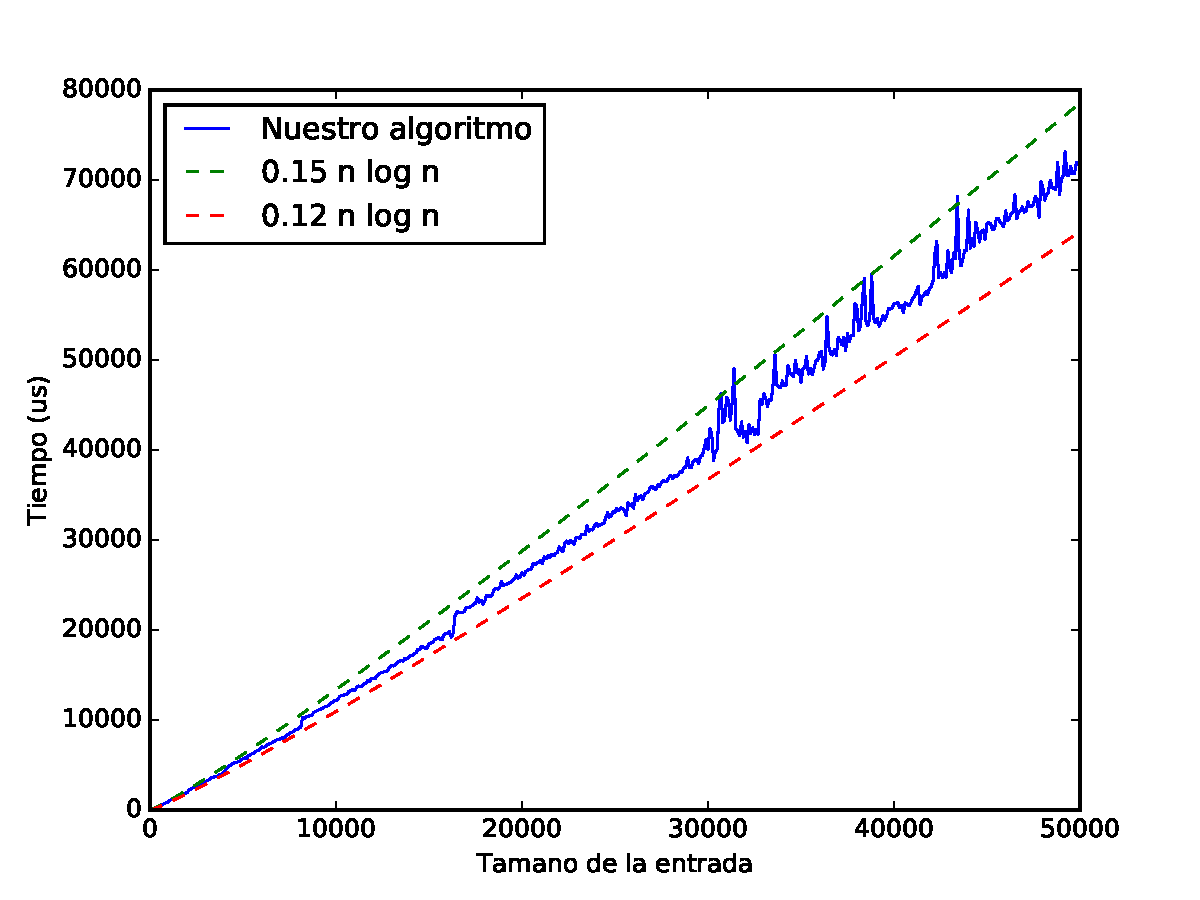
\includegraphics[width=0.8\textwidth]{img/tiempos/kaioken3.pdf}
	\caption{\footnotesize Tiempo que toma el algoritmo en $\mu$s para una entrada de tamaño $n$.}
	\label{fig:kaioken-tiempos3}
\end{figure}

Se ve claramente en la figura \ref{fig:kaioken-tiempos3} que el tiempo que toma el algoritmo esta acotado por arriba y por debajo por $k n \log n$ para algún $k$, es decir, el algoritmo es $\Theta(n \log n)$.

Para hacer un análisis más fino e interesante, es necesario hacer un \emph{close-up} y ver las complejidades de mas cerca.

\begin{figure}[H]
 \centering
	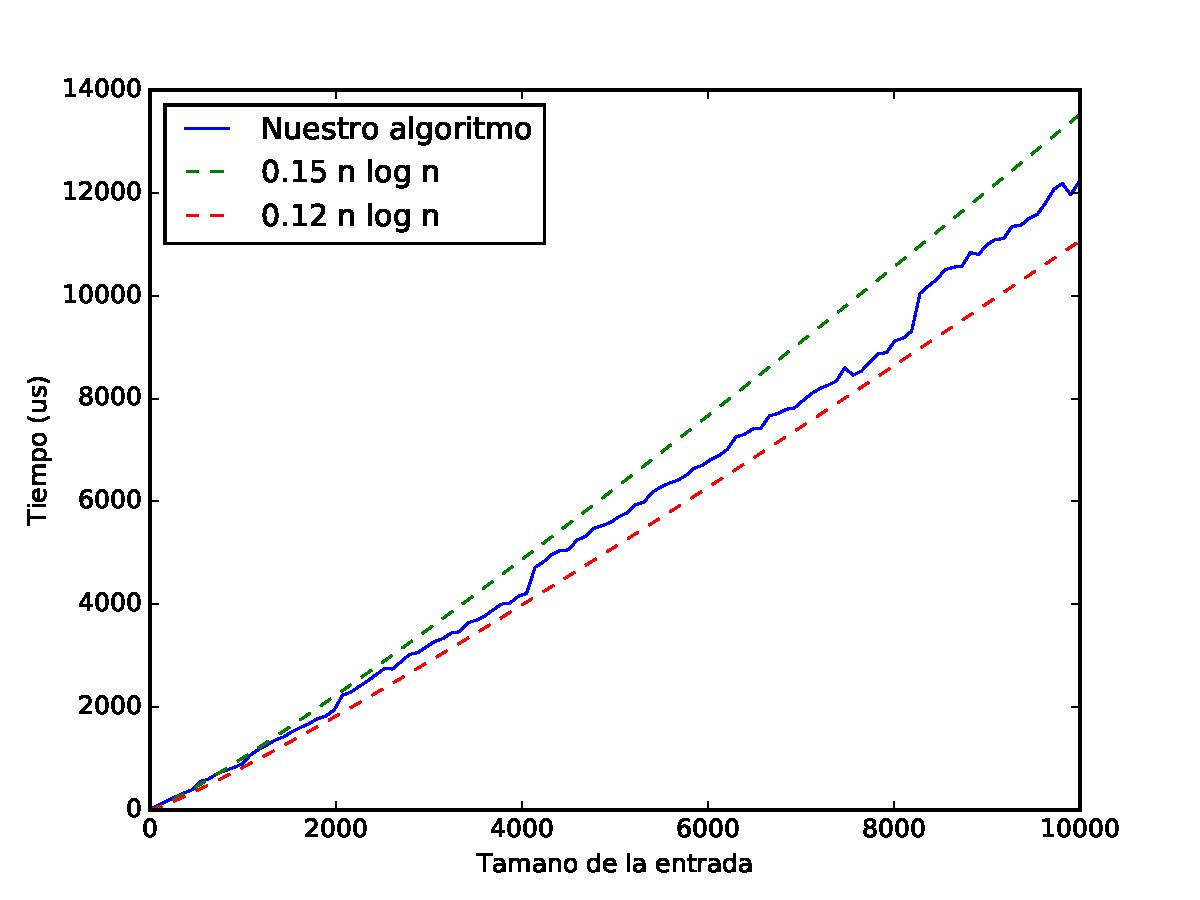
\includegraphics[width=0.8\textwidth]{img/tiempos/kaioken1.pdf}
	\caption{\footnotesize Tiempo que toma el algoritmo en $\mu$s para una entrada de tamaño $n$.}
	\label{fig:kaioken-tiempos1}
\end{figure}

Como puede verse en la figura \ref{fig:kaioken-tiempos1}, el algoritmo claramente es $\Theta(n \log n)$, pero también puede observarse que hay \emph{saltos} de tiempo en algunos lugares.
Se puede inferir fácilmente que estos saltos suceden en las entradas donde $n = 2^k + 1$ para algún $k$, es decir, cuando $n$ es una potencia de 2 más 1.
Esto se debe a que, como fue explicado antes, la cantidad de peleas necesarias es $\lceil \log_2(n) \rceil$, entonces para todos los números entre dos potencias de 2, la cantidad de peleas requerida es la misma, pero luego de una potencia de 2 esta cantidad de peleas aumenta en 1.
A esto se debe los saltos luego de las potencias de 2.

Para visualizar más claramente este hecho, realizamos el siguiente gráfico, en el que están marcadas las potencias de 2.

\begin{figure}[H]
 \centering
	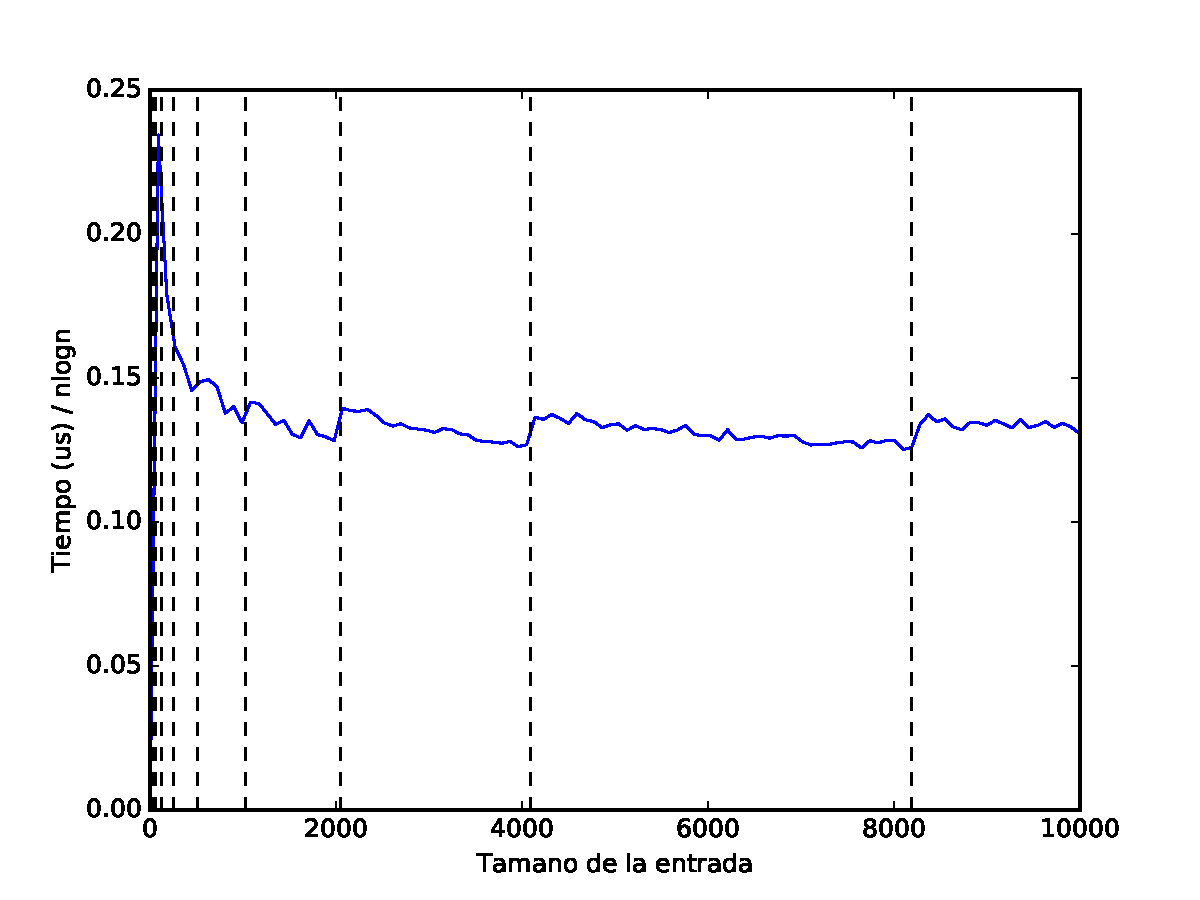
\includegraphics[width=0.8\textwidth]{img/tiempos/kaioken2.pdf}
	\caption{\footnotesize Tiempo que toma el algoritmo en $\mu$s dividido $n\log n$para una entrada de tamaño $n$.}
	\label{fig:kaioken-tiempos2}
\end{figure}

Con la figura \ref{fig:kaioken-tiempos2} se confirma lo que dijimos anteriormente. Luego de cada potencia de 2, el tiempo aumenta, y luego baja lentamente, dado que la relación tiempo - $n \log n$ se mantiene constante, pero $n$ aumenta, con lo cual la división se achica.


\subsubsection{M\'etodo de experimentación}

Para este problema fue muy fácil generar casos de prueba, dado que el único input para el programa es $n$, por lo que simplemente corrimos el programa con diferentes $n$ de entrada. Ejecutamos el programa 50 veces para cada $n$ y el resultado que graficamos fue el mínimo de todas las ejecuciones (para cada $n$). Elegimos el mínimo porque es el que nos permite eliminar outliers que tienen que ver con context switches o con factores de la ejecución sobre los que no tenemos control.



\newpage

\section{Genkidama}
\subsection{Explicación formal del problema}

El ejercicio tiene una bella historia detrás pero a la hora de pensar el problema resulta útil abstraernos un poco y pensarlo en términos de objetos matemáticos. Sobre el plano tenemos un conjunto de puntos $ \{ (X_1,Y_1), (X_2,Y_2), (X_3,Y_3),..., (X_n,Y_n) \} $ todos sus elementos cumplen que $X_1 > X_2 > ... > X_n \geq 0 $ y $ 0 \leq Y_1 < Y_2 < .. < Y_n $. O sea están todos repartidos en el primer cuadrante y formando una especie de escalera decreciente de izquierda a derecha. El objetivo es cubrir a todos los puntos con la menor cantidad de rectángulos que cumplan que sus lados son paralelos a los ejes y sus extremos están en $ (0,0) $ y $ (X_i + T, Y_i + T) $. Donde T es una número entero pasado como parámetro y $(X_i,Y_i)$ son las coordenadas de algún punto del conjunto.

Esto se debe resolver en $ O(n)$ y expresar cuales puntos del conjunto se utilizan como extremos de los rectángulos.

Veamos algunos ejemplos de soluciones correctas e incorrectas para terminar de entender lo que plantea el ejercicio. Analicemos el conjunto de puntos $\{(4,2),(3,3),(2,4),(1,5)\}$ y T = 1.

\begin{figure}[H]
\centering
\begin{minipage}{0.49\textwidth}
  \centering
    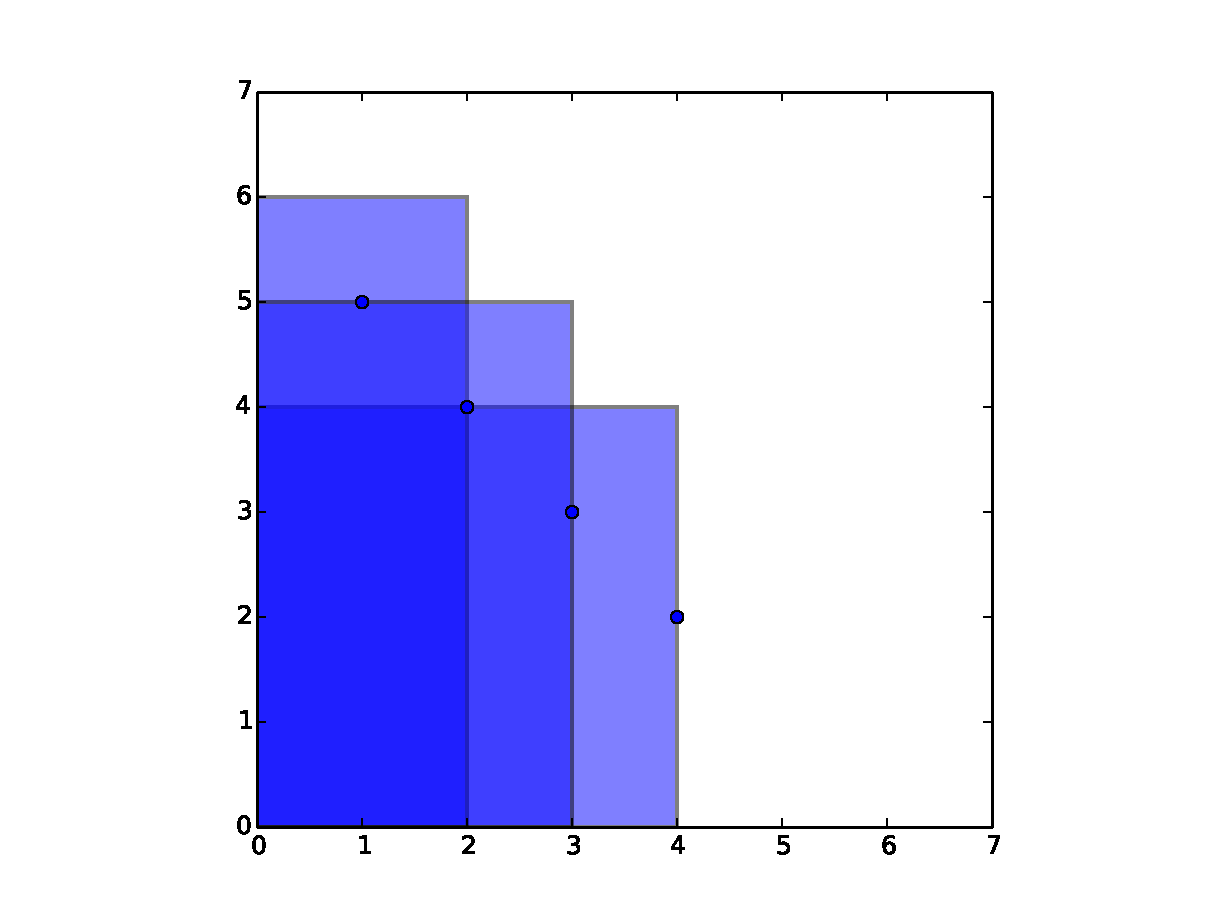
\includegraphics[width=1\textwidth]{img/ejemplos/ej2-1.pdf}
  \caption{\footnotesize Posible elección de rectangulos no óptima.}
  \label{fig:ej3-1}
\end{minipage}%
\hspace{0.01\textwidth}
\begin{minipage}{0.49\textwidth}   
  \centering
    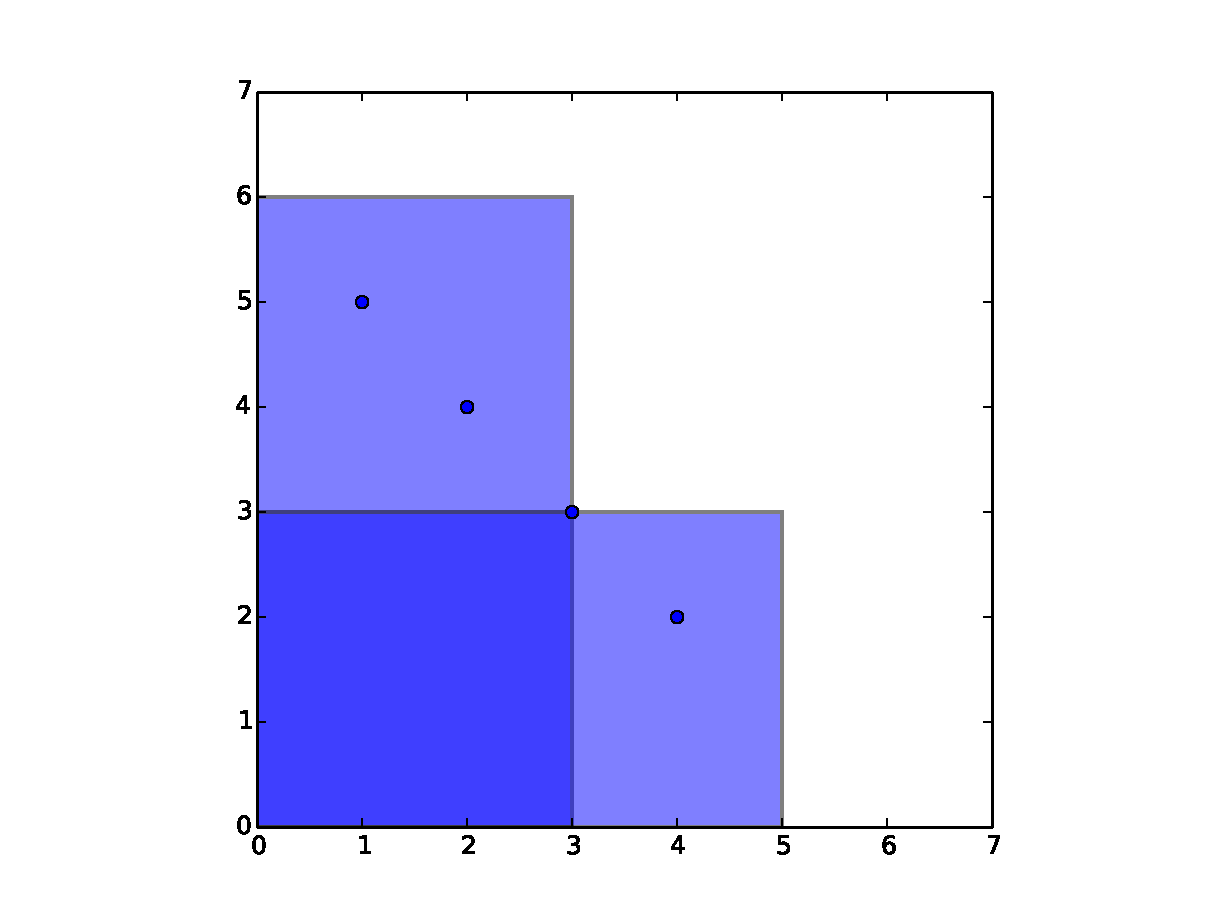
\includegraphics[width=1\textwidth]{img/ejemplos/ej2-2.pdf} 
  \caption{\footnotesize Posible elección de rectangulos incorrecta.}
  \label{fig:ej3-2}
\end{minipage}%
\end{figure}

Algunos ejercicios pueden tener varias soluciones posibles. En este caso tenemos estas dos posibilidades.

\begin{figure}[H]
\centering
\begin{minipage}{0.49\textwidth}
  \centering
    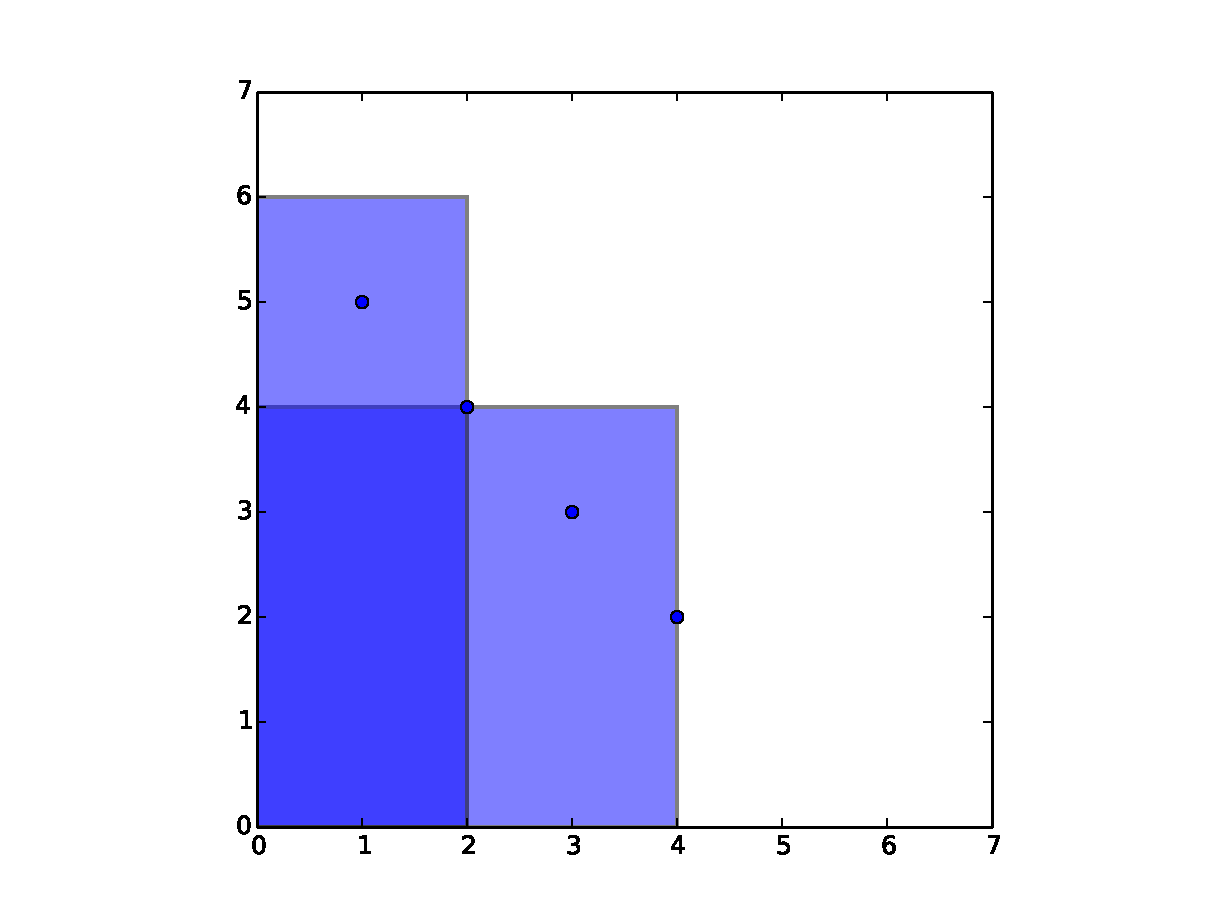
\includegraphics[width=1\textwidth]{img/ejemplos/ej2-3.pdf}
  \caption{\footnotesize Posible elección de rectangulos óptima y correcta.}
  \label{fig:ej3-1}
\end{minipage}%
\hspace{0.01\textwidth}
\begin{minipage}{0.49\textwidth}   
  \centering
    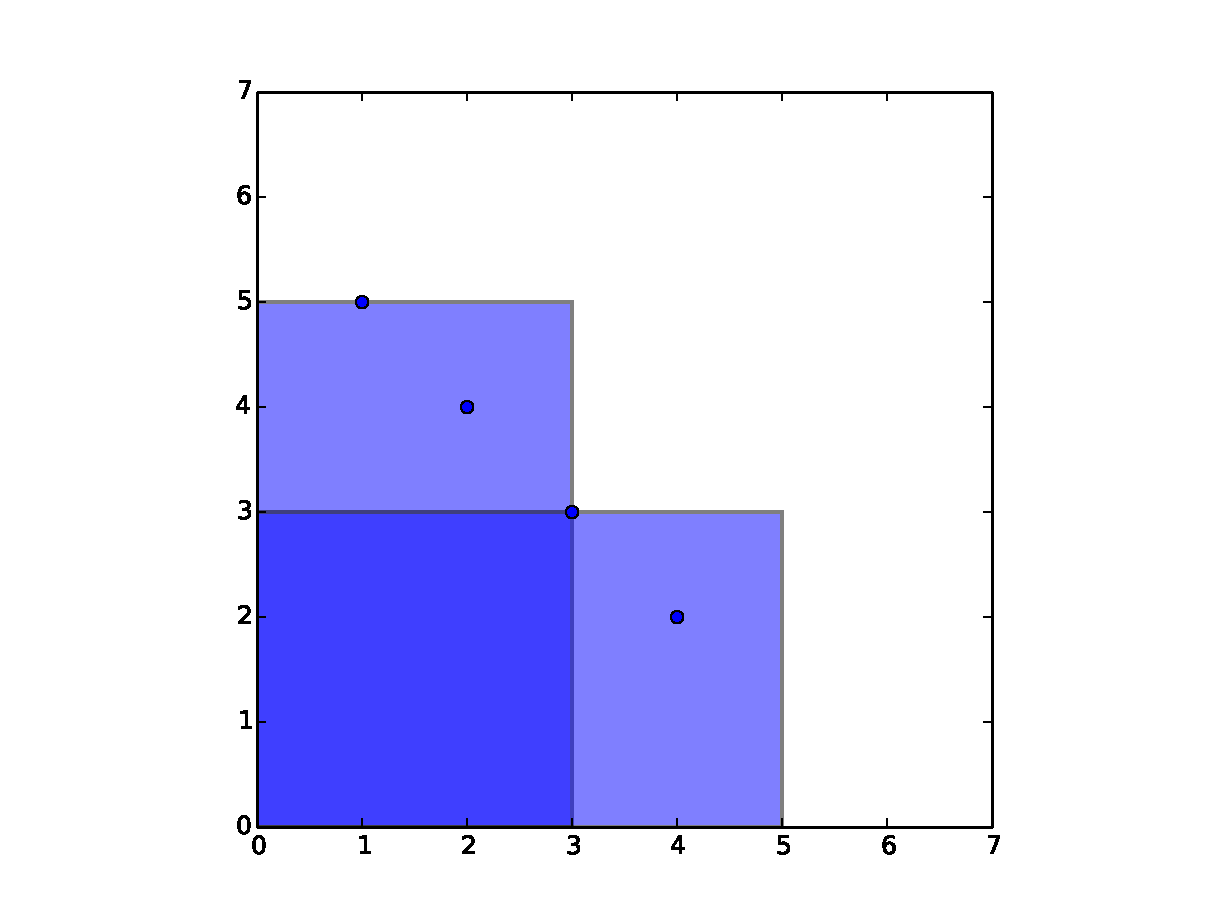
\includegraphics[width=1\textwidth]{img/ejemplos/ej2-4.pdf} 
  \caption{\footnotesize Posible elección de rectangulos óptima y correcta.}
  \label{fig:ej3-2}
\end{minipage}%
\end{figure}


\subsection{Explicación de la solución}

Para resolver el ejercicio utilizamos un $algoritmo$ $goloso$. La idea es ir cubriendo todos los puntos de derecha a izquierda utilizando la menor cantidad de rectángulos posible. La técnica que utilizaremos para lograr esto, la cual veremos luego que es óptima, será por cada iteración del algoritmo buscar un rectángulo que cubra al punto mas a la derecha y al mismo tiempo cubra a la mayor cantidad posible de otros puntos, o sea en cada iteración intentará hacer lo mejor posible para ese momento en particular, por eso lo $greedy$ o $goloso$.

Para la implementación del algoritmo tenemos como datos de entrada los puntos y el valor de $T$, utilizamos una variable $j$ la cual representa el punto mas a la derecha, al cual vamos a cubrir si o si en esa iteración y una variable $i$ la cual representa el candidato a extremo del rectángulo. Comenzamos por el punto mas a la derecha y vamos siguiendo hacia los que tienen una coordenada x menor. Como sabemos que los puntos cumplen que $X_1 > X_2 > ... > X_n \geq 0$ entonces simplemente arrancamos por $X_1$ y seguimos hasta $X_n$, esto se hace fácilmente recorriendo el vector $puntos$ desde su posición $0$ hasta $n-1$. El ciclo principal se encarga de buscar en cada iteración el mejor punto para utilizar como extremo de rectángulo y termina cuando j alcanza a n, lo cual implica que ya se cubrieron todos los puntos.

Veamos el pseudocódigo para que termine de quedar claro todo esto. Las guardas de los dos ciclos anidados las omito y detallo mas abajo.

\begin{algorithm}[H]
\begin{algorithmic}
\caption{Esbozo del algoritmo de Genkidama}
  \Procedure{aQuienDisparo}{vector(int,int) $puntos$, int $t$}
	\State int n = puntos.cantidad()
	\State int i = 0
	\State int j = 0
    \While {$j < n$}
    		\State i = j
		\While { $...$ }
			\State $ i++ $
	  	\EndWhile
		\State $respuesta.agregarA(i)$
		\State $ i++ $
		\While { $ ... $ }
			\State $ j++ $
	 	\EndWhile
  \EndWhile
  \EndProcedure
\end{algorithmic}
\end{algorithm}

Para lograr hacer lo dicho previamente el ciclo principal cuenta con dos bucles anidados.

El primer ciclo tiene como objetivo cubrir a j y al mismo tiempo verificar si no puede cubrir algunos mas. En el pseudocódigo se puede ver fácilmente como hacemos eso.

\begin{algorithm}[H]
\begin{algorithmic}

\caption{Ciclo Anidado 1}

\While { $ i < n - 1 \land puntos[i+1].primero + t \geq puntos[j].first $ }
	\State $i++$
\EndWhile

\end{algorithmic}
\end{algorithm}

Si podemos cubrir a un punto mas al mismo tiempo que seguimos cubriendo al punto $(X_i,Y_i)$ entonces guardamos ese nuevo valor como nuestro nuevo candidato para utilizar como extremo del nuevo rectángulo. Repetimos esto hasta que ya consideramos todos los puntos o que el siguiente a nuestro candidato ya no nos permite cubrir a $(X_i,Y_i)$.

Cuando conseguimos al mejor candidato, lo almacenamos y seguimos con el Ciclo Anidado 2.

El segundo ciclo tiene como tarea verificar si al haber agregado el nuevo rectángulo no se cubrieron algunos puntos mas a la izquierda.

\begin{algorithm}[H]
\begin{algorithmic}

\caption{Ciclo Anidado 2}

\While { $ j < n \land puntos[j].segundo \leq puntos[i-1].segundo + T $ }
	\State $j++$
\EndWhile

\end{algorithmic}
\end{algorithm}

En ese caso se aumenta $j$ para que pase a representar al siguiente punto. Se repite esto hasta encontrar uno punto que no haya sido cubierto todavia o hasta que no hayan mas puntos.

\subsubsection{Optimalidad}

Para demostrar que el algoritmo propuesto es óptimo supondré que no lo es y llegaré a un absurdo. Supongamos que tenemos una solución que es óptima, sabemos que esta existe ya siempre podemos encontrar entre todas las finitas (no nulas) formas de cubrir todos los puntos con rectángulos la que use la menor cantidad. Sabiendo que esta solución es óptima entonces de seguro tiene que tener algo distinto a lo que devuelve nuestro algoritmo ya que supusimos que no era óptimo, tiene que tomar al menos una decisión distinta en la elección de los rectángulos.

Dada la solución que sabemos es óptima, nos ponemos a ver las elecciones de rectángulos que la componen de derecha a izquierda. O sea viendo primero al que tiene como extremo al punto de mayor coordenada x y siguiendo hacia los menores.

Al ponernos a ver las elecciones de rectángulos que hay en la solución óptima en algun momento vamos a notar se escoge tapar al punto que estaba mas abajo a la derecha pero sin tapar al mismo tiempo a la mayor cantidad posible de otros puntos sin cubrir. Sabemos que esto va a pasar en algun momento ya que si no fuera así entonces sería exactamente igual a la solución de nuestro algoritmo.

Pero al ver esto se vuelve obvio que esa desición es peor o igual que lo que hacemos, ya que con nuestro algoritmo podriamos reemplazar esa acción por una que cubrá una mayor cantidad de puntos. Terminando en el peor de los casos usando la misma cantidad de rectángulos para la solución. Lo cual es absurdo ya que habiamos supuesto que nuestro algoritmo no era óptimo.

\subsection{Complejidad del algoritmo}

En esta sección demostraremos que el algoritmo tiene una complejidad de $\Theta(n)$ donde n es la cantidad de puntos en el plano para cualquier caso (no existe peor ni mejor caso). O sea eventualmente, cuando n crece lo suficiente, la cantidad de instrucciones elementales queda acotada inferiormente por $k_1.n$ y superiormente por $k_2.n$ con $k_1$ y $k_2$ alguna constante real fija.

Para demostrar lo dicho analicemos las partes que componen a este programa. Primero se crean variables lo cual cuesta a lo sumo $O(n)$, dependiendo la estructura utilizada, por tener que averiguar la cantidad de puntos en el vector de entrada.

Lo siguiente es el ciclo principal el cual veremos que toma $\Theta(n)$. Veamos una serie de proposiciones que utilizaré para demostrarlo, todas son evidentes viendo el pseudocódigo.

\begin{enumerate}

\item Los ciclos 1 y 2 cuestan $O(1)$ por iteración.

\item La variable j aumenta una vez por cada iteracion de cada ciclo en que entra. (En cualquier de los 3 ciclos que hay).

\item Si j vale n entonces terminan todos los ciclos.

\end{enumerate}

Por (3) sabemos que el ciclo solo funcionara mientras j sea menor a n, mientras esto se cumpla se iterara en el ciclo principal y por (1) sabemos que se gastará una cantidad constante de pasos cada vez que se itere en uno de los ciclos internos, por la proposición (2) sabemos que al final de cada iteración del ciclo principal el valor de j será aumentado la cantidad de veces que haya ciclado dentro del primer ciclo anidado mas la cantidad de veces que lo haya hecho en el segundo ciclo anidado mas uno por la iteración principal. Si este valor llega a n el ciclo terminará. Si no ocurre entonces se hará una iteración mas en el ciclo principal. Por lo tanto vamos gastando O(1) cada vez que incrementamos en 1 a j. Y j termina cuando vale n por lo tanto este algoritmo tarda $\theta(n)$, solo nos podemos pasar de ese costo si j llega a valer mas de n y eso no puede pasar por la proposición (3). Tampoco vamos a tardar menos que eso por que eso significaría que j vale menos de n y no puede terminar en ese caso.

Habiendo demostrado esto, sumado a que las instrucciones fuera del ciclo son todas a lo sumo O(n) queda demostrado que la función esta acotada superior e inferiormente por n, para cualquier caso.

\subsection{Performance del algoritmo}

Como vimos anteriormente, el algoritmo tiene una complejidad de $\Theta(n)$. El algoritmo no tiene peor o mejor caso propiamente dichos (dado que es $\Theta(n)$ para todos los casos), pero veremos que las constantes pueden cambiar para algunas entradas por cuestiones de implementación.

\begin{figure}[H]
 \centering
	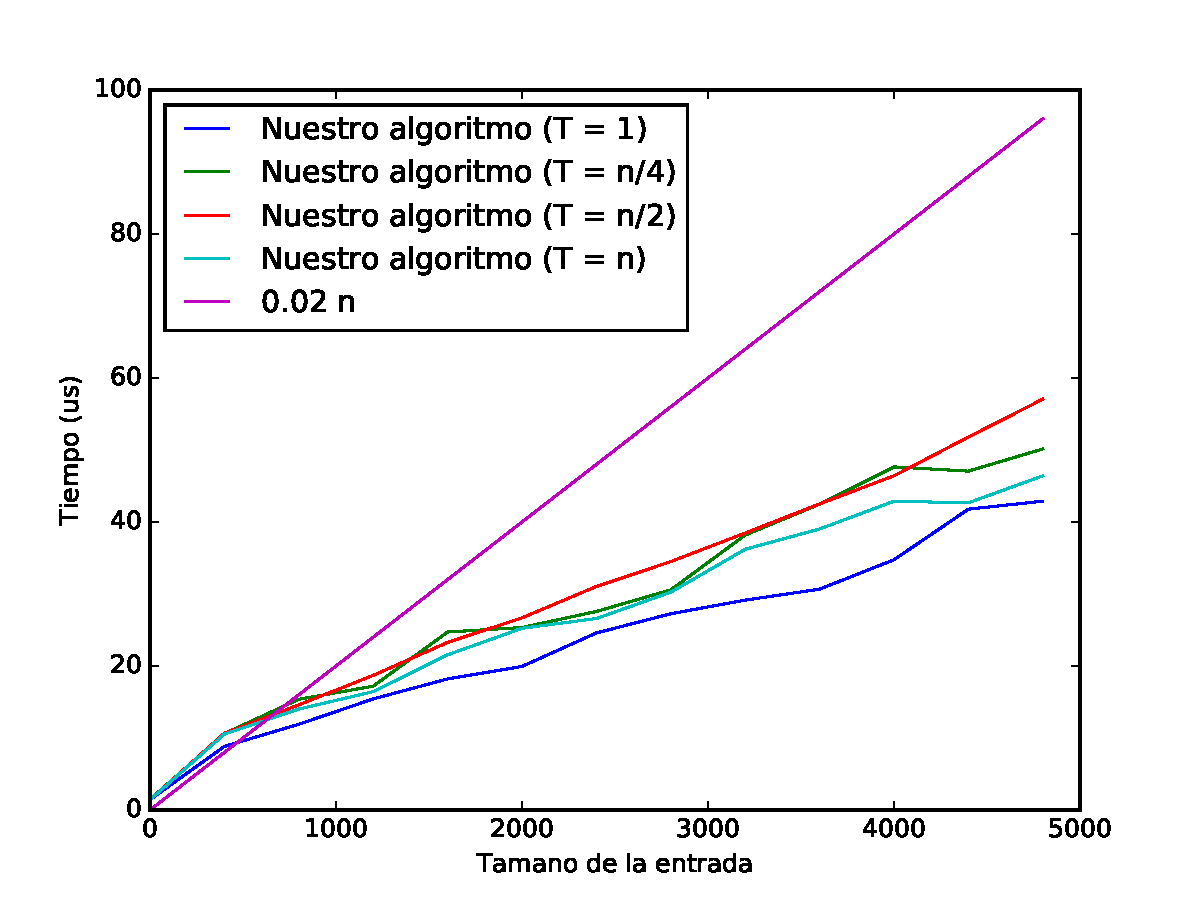
\includegraphics[width=0.8\textwidth]{img/tiempos/genkidama1.pdf}
	\caption{\footnotesize Tiempo que toma el algoritmo en $\mu$s para una entrada de tamaño $n$.}
	\label{fig:genkidama-tiempos1}
\end{figure}

Como se observa, la implementación tiene complejidad lineal, como era esperado. Sin embargo, se observan diferencias según el $T$ que se elija. Recordemos que el $T$ era el radio de impacto del genkidama. Esto se debe a una cuestión de implementacion. Para los casos donde $T = 1$ o $T = n$, nuestra implementación se ahorra entrar a un while, reduciendo la cantidad de instrucciones que ejecuta cada vez.

\begin{figure}[H]
 \centering
	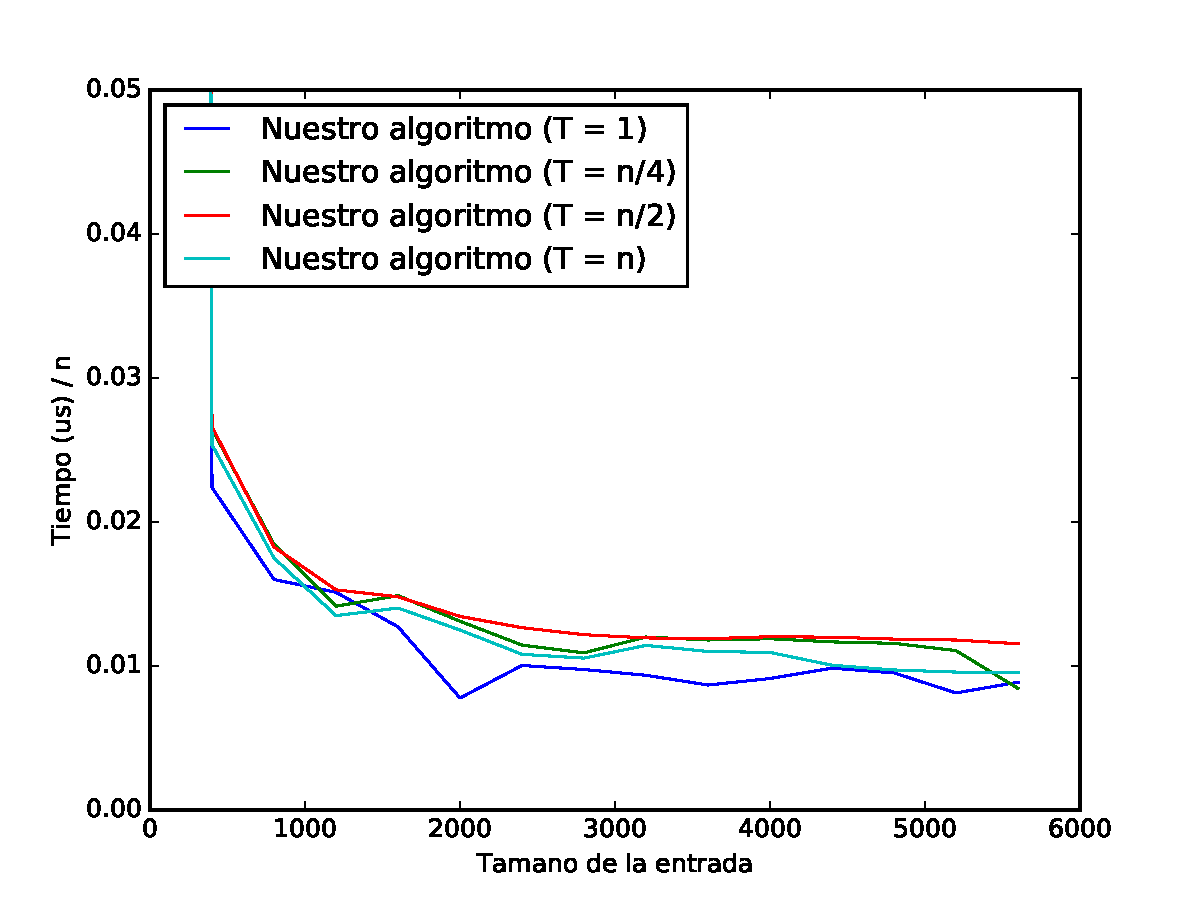
\includegraphics[width=0.8\textwidth]{img/tiempos/genkidama2.pdf}
	\caption{\footnotesize Tiempo que toma el algoritmo en $\mu$s dividido $n$ para una entrada de tamaño $n$.}
	\label{fig:genkidama-tiempos2}
\end{figure}

Este gráfico nos ayuda aún más a confirmar la complejidad lineal de este algoritmo, ayudandonos a ver las constantes para cada caso. Nuevamente, observamos que el caso $T = 1$ tiene una constante un poco menor, debido a lo explicado anteriormente.

Finalmente, veamos que, para instancias de igual tamaño, el tiempo que se tarda en resolverlas no varía demasiado (confirmando el hecho de que para $T$ fijo, la elección de los puntos no cambia el tiempo de ejecución de manera significativa).

\begin{figure}[H]
 \centering
	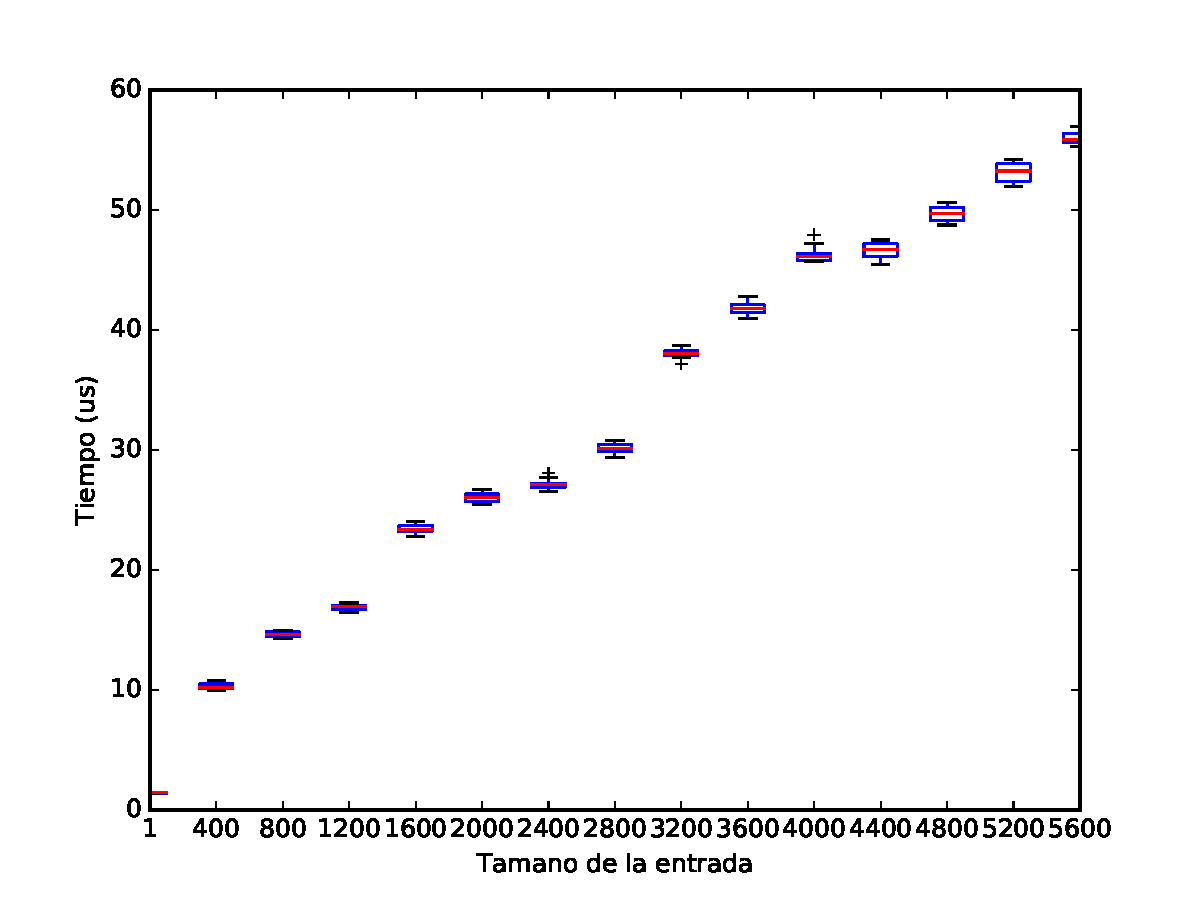
\includegraphics[width=0.8\textwidth]{img/tiempos/genkidama3.pdf}
	\caption{\footnotesize Tiempo que toma el algoritmo en $\mu$s para una entrada de tamaño $n$. $T = n/4$. Se indican los valores del primer al tercer cuartil con un rectángulo azul y la mediana con una linea roja. El máximo y minimo se indican con lineas negras arriba y abajo del rectángulo.}
	\label{fig:genkidama-tiempos3}
\end{figure}

\subsubsection{M\'etodo de experimentación}

Para los primeros dos gráficos (es decir, para la figura \label{fig:genkidama-tiempos1} y la figura \label{fig:genkidama-tiempos2}), generamos 50 instancias al azar de para cada $n$.
Las instancias fueron generadas de la siguiente manera: para cada $n$, elegimos $n$ puntos al azar de la grilla $\{1,..., n^2\} \times \{1, ... , n^2\}$.
Estos puntos eran elegidos al azar usando el mismo \emph{seed} cada vez (para la instancia 1 usábamos 1 como seed, para la instancia 2, usábamos 2, etc.), de tal manera que los experimentos fueran reproducibles de una manera válida.

Cada instancia fue ejecutada 20 veces, y el resultado final era el mínimo de todas las corridas.
Luego, tomabamos la mediana de todas las instancias.
Es decir, el resultado final es la mediana de los mínimos. Como puede observarse en la figura \ref{fig:genkidama-tiempos3}, la mediana es muy representativa de lo que sucede.

\newpage

\section{Kamehameha}
\subsection{Explicación formal del problema}
\label{subsec:problema3}
Sea el conjunto de puntos del primer cuadrante $C = \{(x_1, y_1), \hdots, (x_n, y_n)\}$. Se desea hallar alguna partición, $P$, del mismo que tenga cardinalidad mínima y cumpla la siguiente condición: $(\forall X \in P) (\exists r$ : semirrecta$) (\forall punto \in X)$ $punto \in r$. Esto es, que cada conjunto de la partición solo puede tener puntos que pertenecen a una misma semirrecta (sea cual sea esta). 
Notar que la segunda condición no restringe la posibilidad de que $r$ atraviese puntos de otro conjunto de la partición. 
%También ver que por la primer condición (cardinalidad mínima), si $r'$ es la semirrecta correspondiente a $X'$, no puede ocurrir que $r' \subset r$ pues en tal caso considero la partición $P'$, igual a $P$ salvo porque tengo $X'' = X \cup X'$ (que cumple la segunda condición dado que $r$ verifica bien) en lugar de $X$ y $X'$, y por tanto tiene cardinalidad estrictamente menor que $P$, lo que conduce a un absurdo. 

Por ejemplo, consideremos $C=\{(3,2), (3,5), (3,7), (5,6), (7,4)\}$. Tomemos la partición $P' = \{\{(3,2), (3,5)\}, \{(3,7)\}\},\{(5,6), (7,4)\}\}$. Para ver si $P'$ es solución de nuestro problema grafiquemos los puntos y trazemos una posible configuración de semirrectas correspondiente a la partición, como en la figura (\ref{fig:ej3-2})\footnote{En esta sección los gráficos usarán la siguiente convención: los puntos considerados están marcados con círculos y cuadrados, representando estos últimos el origen de las semirrectas. }. Viendo esto es claro que podría atravesarse todos los puntos con solo dos semirrectas en lugar de 3. Inspirados en la figura (\ref{fig:ej3-1}) deducimos que una solución es $P = \{\{(3,2), (3,5), (3,7)\},\{(5,6), (7,4)\}\}$. En este caso puntual además resulta que es la única solución posible (teniendo en cuenta que no nos importa el orden de los puntos por ser conjuntos). Aunque esto en general no vale, como se ve por ejemplo en las figuras (\ref{fig:ej3-3}) y (\ref{fig:ej3-4}), donde las elecciones de semirrectas inducen particiones claramente distintas.

\begin{figure}[H]
\centering
\begin{minipage}{0.49\textwidth}
  \centering
    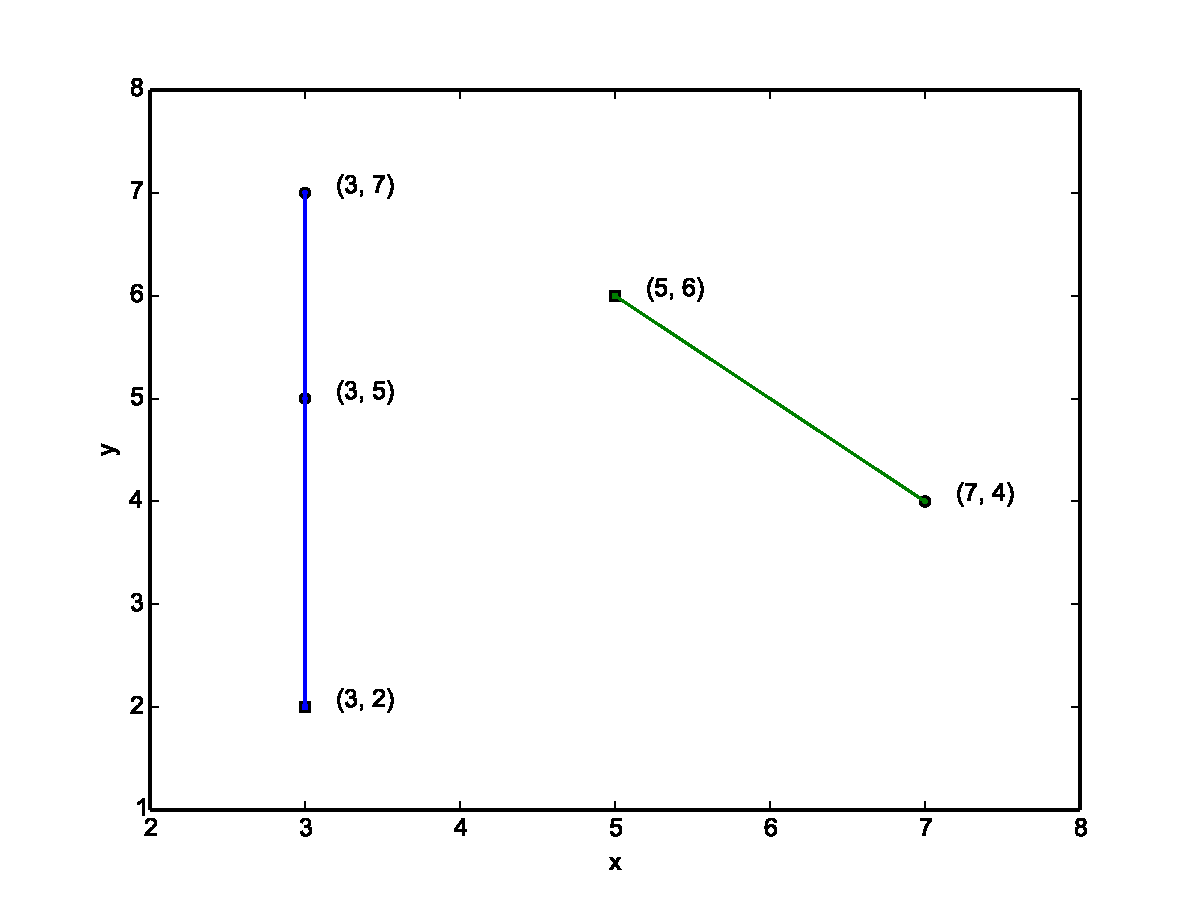
\includegraphics[width=1\textwidth]{img/ejemplos/ej3-1.pdf}
  \caption{\footnotesize Posible elección de semirrectas para la partición $P$.}
  \label{fig:ej3-1}
\end{minipage}%
\hspace{0.01\textwidth}
\begin{minipage}{0.49\textwidth}   
  \centering
    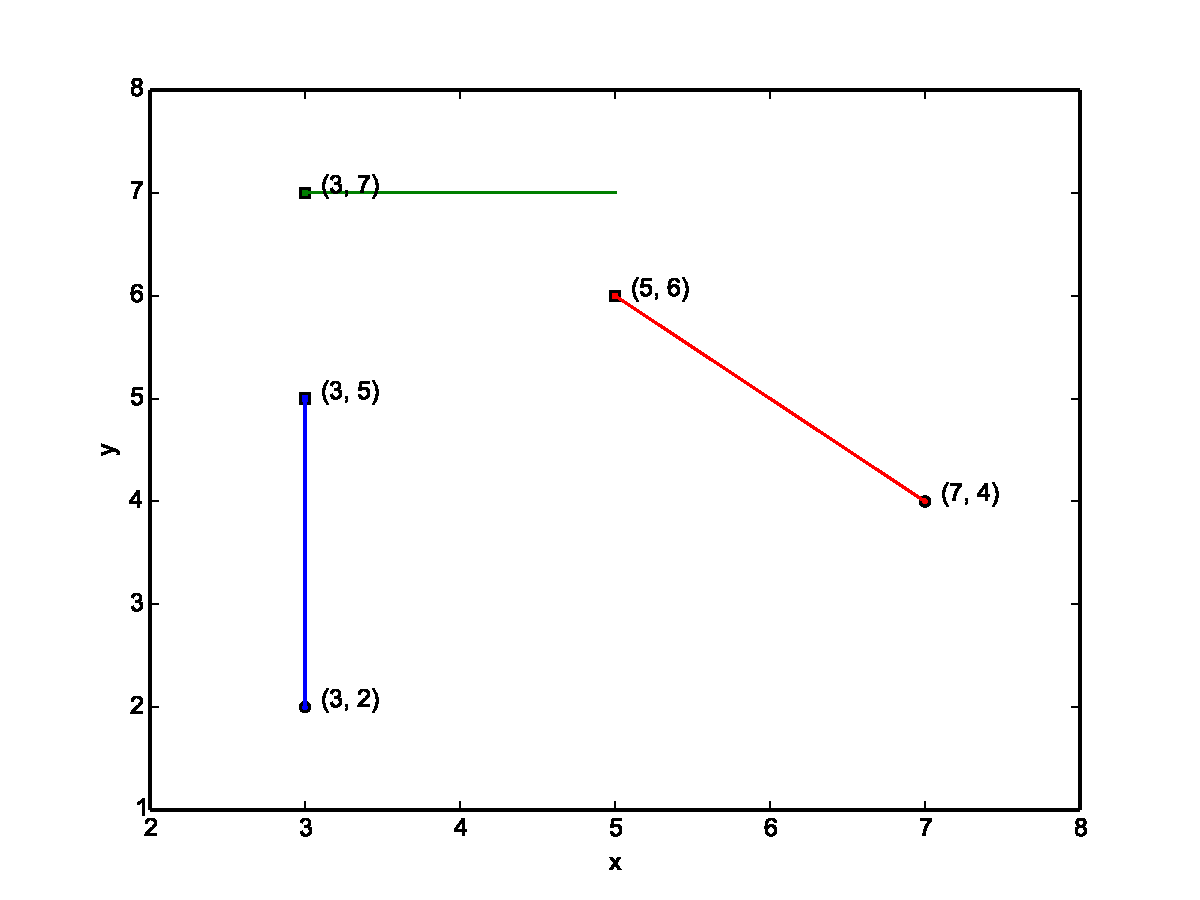
\includegraphics[width=1\textwidth]{img/ejemplos/ej3-2.pdf} 
  \caption{\footnotesize Posible elección de semirrectas para la partición $P'$.}
  \label{fig:ej3-2}
\end{minipage}%
\end{figure}

\begin{figure}[H]
  \centering
  \begin{minipage}{0.49\textwidth}
  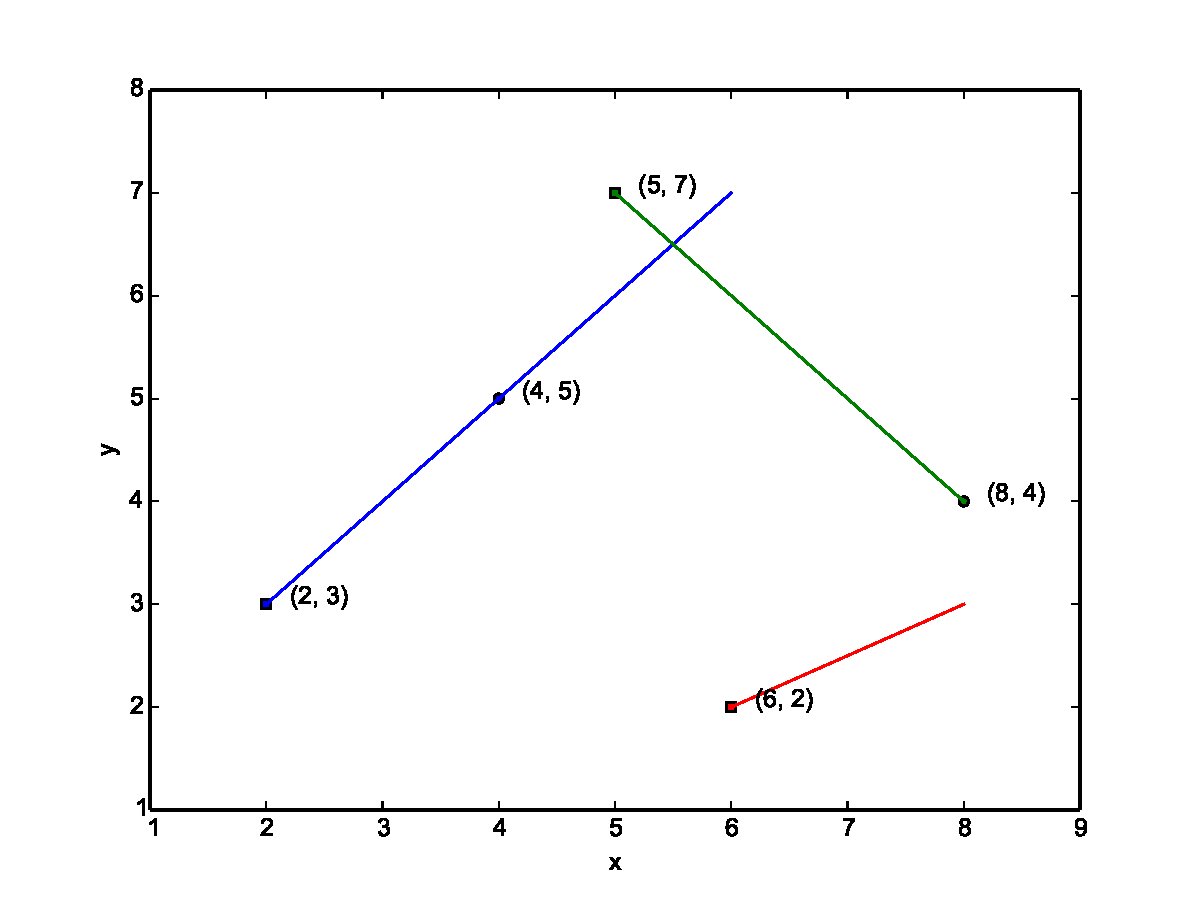
\includegraphics[width=0.75\textwidth]{img/ejemplos/ej3-3.pdf}
  \caption{\footnotesize Solución óptima para un conjunto dado de 5 puntos, donde no hay 3 puntos alineados.}
  \label{fig:ej3-3}
  \end{minipage}%
  \hspace{0.01\textwidth}
  \begin{minipage}{0.49\textwidth}
  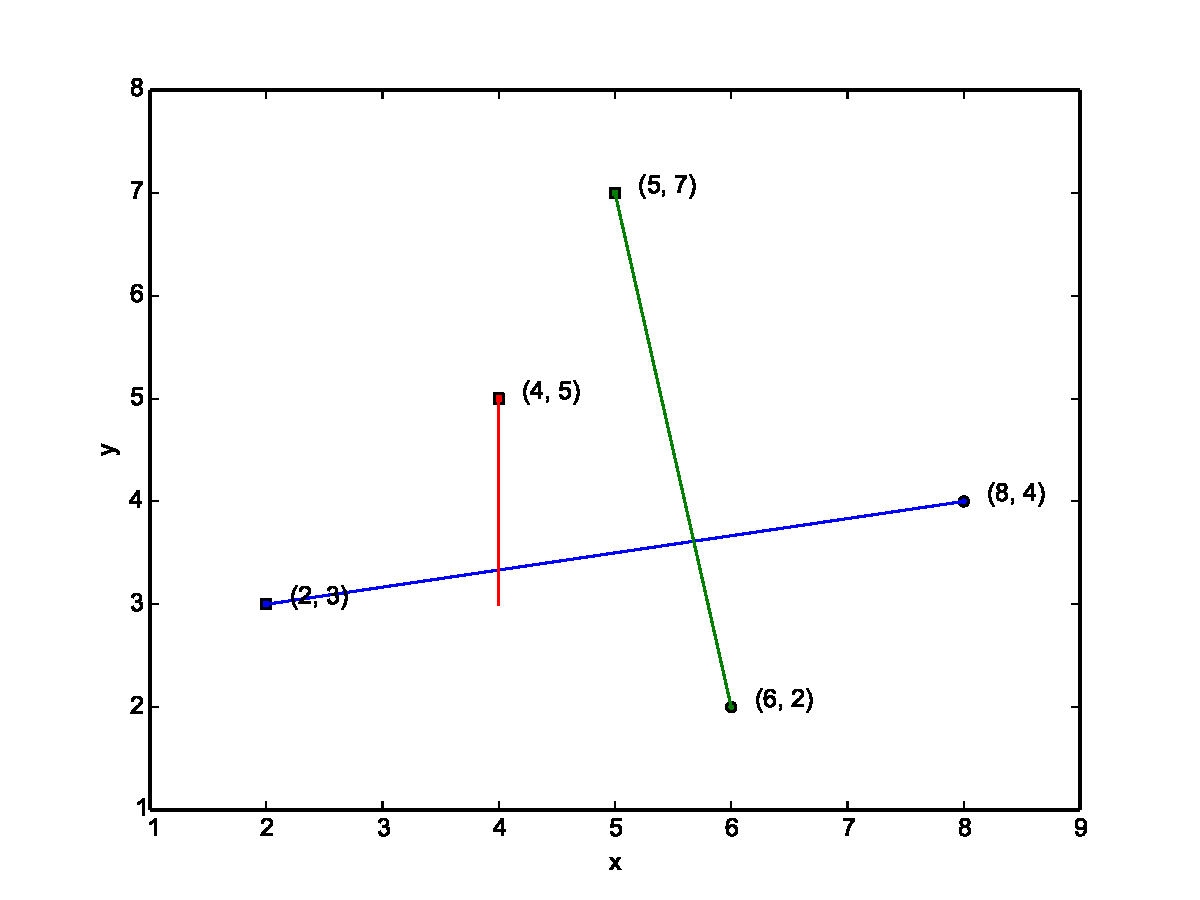
\includegraphics[width=0.75\textwidth]{img/ejemplos/ej3-4.pdf}
  \caption{\footnotesize Solución óptima para un conjunto dado de 5 puntos, donde no hay 3 puntos alineados.}
  \label{fig:ej3-4}
  \end{minipage}%
\end{figure}

Debido a que entre dos puntos siempre se puede establecer un semirrecta que los una, ningún conjunto de la partición solución, $P$, puede tener menos de dos elementos, salvo quizás uno (como ocurre en la figura \ref{fig:ej3-3})). Si tuviera al menos dos conjuntos en $P$ con un solo elemento, $X y X'$, entonces podría considerar $P'$, igual a $P$ salvo que tiene a $X'' = X \cup X'$ (que es válido porque seguro hay una semirrecta que una los dos puntos) y por lo tanto no posee a $X y X'$. Claramente el cardinal de $P'$ es estrictamente menor al de $P$, lo que es un absurdo pues $P$ era solución. Luego, $P$ puede tener a lo sumo un conjunto con un elemento.

Por lo dicho en el párrafo anterior, se puede establecer una cota superior al cardinal de la solución cuando tengo $n$ puntos: $\lceil\frac{n}{2}\rceil$ ¿Cuándo se alcanza dicha cota? Cuando no existe ninguna semirrecta que pueda atravesar más de dos puntos. Una disposición fácil de generar este tipo de casos es considerar $n$ puntos esparcidos sobre una circunferencia (una recta solo puede ser tangente o secante respecto a una circunferencia). En la figura (\ref{fig:ej3-5}) puede verse un ejemplo de esta situación para 16 puntos.

\begin{figure}[H]
  \centering
  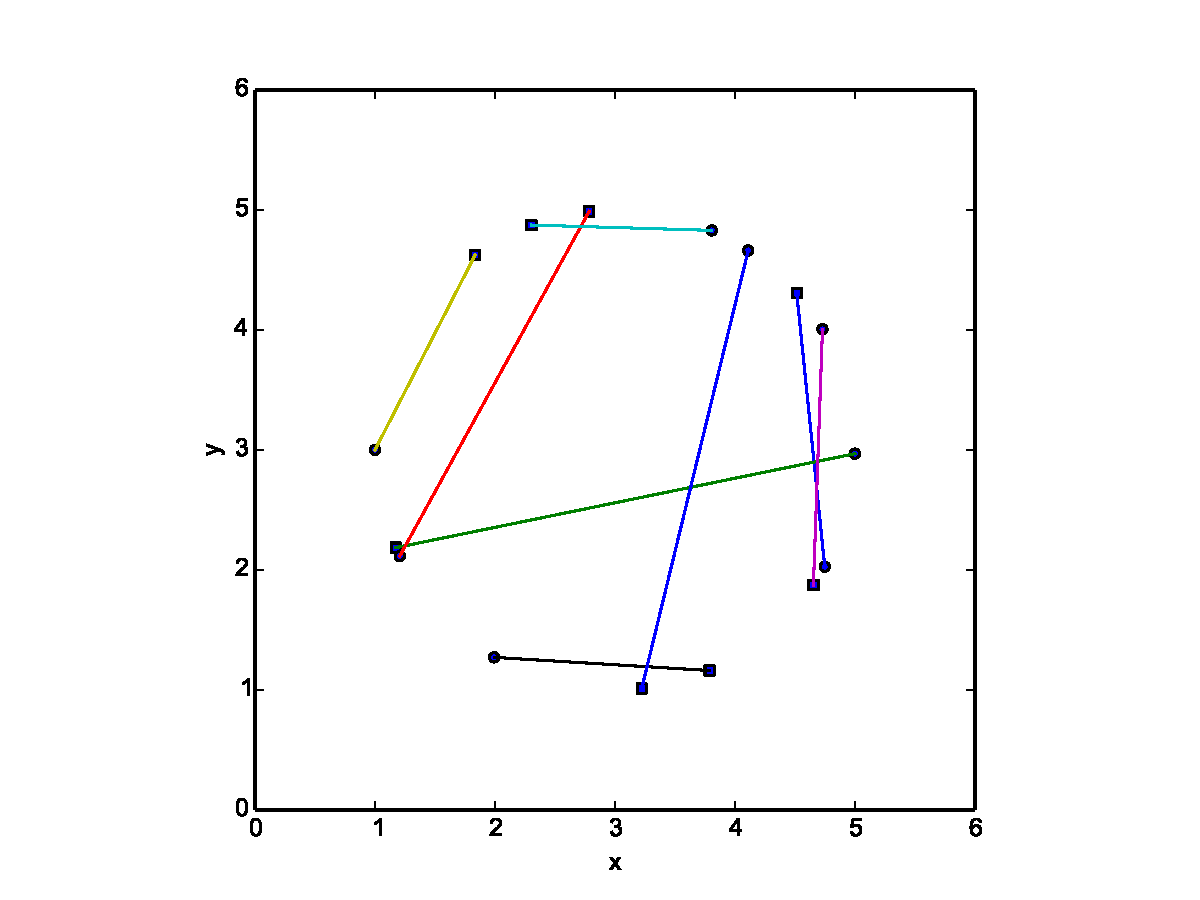
\includegraphics[width=0.70\textwidth]{img/ejemplos/ej3-5.pdf}
  \caption{\footnotesize Solución óptima para un conjunto de 16 puntos dispuestos sobre una circunferencia de radio 2 centrada en $(3,3)$.}
  \label{fig:ej3-5}
\end{figure}

\subsection{Explicación de la solución}
En esta sección daremos una breve explicación de porque el método de \texttt{backtracking} resulta correcto para resolver el problema presentado,  luego contaremos las podas y estrategias utilizadas, y finalmente presentaremos una explicación de las partes fundamentales de la implementación. 

\subsubsection{Árbol de posibilidades}
Los algoritmos de \texttt{backtracking} son un refinamiento de los algoritmos de fuerza bruta por lo que pensemos primero la solución usando este método. Este último tipo de algoritmos consisten en enumerar todos los posibles candidatos a solución del problema y ver si satisfacen las condiciones pedidas o no. En nuestro caso particular, todas los posibles candidatos van a ser las particiones que cumplan la segunda condición del enunciado, y de estas nos quedamos con alguna que tenga cardinal mínimo. 

El proceso de construir las particiones se puede pensar como un árbol en el que en cada nivel se agrega un nuevo conjunto de los posibles a la partición que estoy armando. Así, en el nivel 0 (la raíz) tengo un conjunto vacío. En el nivel 1 tengo todos los subconjuntos de $C$ que verifican que existe alguna semirrecta que los une. Al escoger alguno de estos conjuntos lo agregamos en la potencial partición. Debido a esto, en el nivel 2 tenemos un subconjunto de las posibilidades del nivel 1 estrictamente más pequeño pues debemos eliminar todas aquellas opciones que involucraban alguno de los puntos presentes en el conjunto previamente agregado (los conjuntos de la partición deben ser disjuntos). Se repite un procedimiento análogo hasta completar la partición, momento en el que estaremos parados en una hoja del árbol. 

Haciendo DFS (Depth-first search) recorremos todo el árbol de posibilidades, de forma que finalmente encontramos todas las particiones que cumplen la condición dos. Finalmente nos quedamos con alguna de cardinal mínimo (si hubiera más de una).

La correctitud de tal algoritmo es clara pues encuentra todo el universo de posibles soluciones, por lo que si efectivamente existe alguna eventualmente la obtiene. En particular, para todo conjunto finito es posible establecer particiones, así que siempre hay solución. 

La idea de \texttt{backtracking} es preservar esta garantía de correctitud pero agilizando la búsqueda mediante la utilización de podas en el árbol de posibilidades. Dicho de otra forma, un algoritmo de este tipo descarta \texttt{candidatos a soluciones parciales} que a partir de algún criterio podemos predecir que no nos van a conducir a la solución. En nuestro problema, un candidato a solución parcial es una partición en construcción. En la siguiente sección mostramos con que criterios los descartamos.

\subsubsection{Podas realizadas}
\begin{enumerate}
  \item Si actualmente estamos parados en un nodo de nivel $s$ (es decir que el cardinal de nuestro candidato a solución parcial es $s$) y anteriormente ya habíamos encontrado una solución en el nivel $s$, entonces no tiene sentido continuar por ese camino pues sabemos que todas los candidatos a soluciones a los que se arrive van a ser peores que un candidato previamente encontrado. De esta forma estamos ahorrándonos una búsqueda innecesaria y potencialmente muy costosa.
  \item Por lo observado en la sección \ref{subsec:problema3}, no tiene sentido considerar agregar conjuntos que tienen un solo elemento, salvo potencialmente en el último paso. Esto elimina muchas ramas del árbol.
\end{enumerate}

\subsubsection{Pseudocódigo}
  \begin{algorithm}[H]
  \begin{algorithmic}
  \caption{Pseudocódigo del procedimiento de \texttt{backtracking} en Kamehameha}
    \Procedure{backtracking}{Tablero $t$, int $step$}
    \If {$step \geq mejor$}
      \State $return$
    \EndIf
    \If {$t.Solucionado()$}
      \State $mejor \gets step$
      \State $mejor\_sol \gets t.Solucion()$
    \Else
      \For {$i \in [0,..., n),$ $t.EstaVivo?(i)$}
        \If {$t.SoloQuedaUno?()$}
          \State $t.Matar(i)$
          \State $backtracking(t, step+1)$
          \State $return$
        \EndIf
        \For {$j \in [0,..., n),$ $j \neq i \land t.EstaVivo?(j)$}
          \State $Tablero$ $sucesor \gets Copiar(t)$
          \State $Vector(int)$ $derrotados \gets [i, j]$ 
          \For {$k \in [0,..., n),$ $k \neq i \land k \neq j \land t.EstaVivo?(k)$}
            \If {$x_i \neq x_j \land y_i \neq y_j$}
              \If {$\frac{x_k-x_i}{x_j-x_i} = \frac{y_k-y_i}{y_j-y_i} \land MismoCuadrante?(i,j,k)$}
                \State $derrotados.AgregarAtras(k)$
              \EndIf
            \Else 
              \If {\small{$(AlinHor?(i,j,k) \lor AlinVer?(i,j,k)) \land MismoCuadrante?(i,j,k)$}}
                \State $derrotados.AgregarAtras(k)$
              \EndIf
            \EndIf
          \EndFor
          \State $sucesor.Matar(derrotados)$
          \State $backtracking(sucesor, step+1)$
        \EndFor
      \EndFor
    \EndIf
    \EndProcedure
  \end{algorithmic}
  \end{algorithm}

\subsection{Complejidad del algoritmo}

\subsection{Performance del algoritmo}
\newpage
\section{Apéndice}
\subsection{Demostración del Lema 3.1}

Vamos a demostrar que $T(n) = F(n)$, si $n=2k$ con $k\in\mathbb{N}$, por inducción en $k$.

\textbf{Caso base:} $k=0 \implies n=0$

  $T(0) = 1$ 

  Dado que las sumatorias y las productorias en las que el límite inferior es más grande que el superior se devuelve el elemento neutro para la suma y el producto, 0 y 1 respectivamente, tenemos que $F(0) = 1$. Entonces demostramos el caso base.

\textbf{Paso inductivo:} Supongamos que $T(n) = F(n)$. Veamos que también vale $T(n + 2) = F(n + 2)$ \\
  \begin{equation}
  \label{eq:ind3-1}
  \begin{aligned}
  T(n+2) &= (n+2)^3 + (n+2)^2 T(n) \\
         &= (n+2)^3 + (n+2)^2 F(n) \\
         &= (n+2)^3 + (n+2)^2 \sum_{i=0}^{\frac{n}{2}-1} \left((n-2i) \prod_{j=0}^{i}(n-2j)^2\right) + (n+2)^2 \prod_{i=0}^{\frac{n}{2}-1}(n-2i)^2\\
         &= (n+2)^3 + \sum_{i=0}^{\frac{n}{2}-1} \left((n-2i) (n+2)^2 \prod_{j=0}^{i}(n-2j)^2\right) + (n+2)^2 \prod_{i=0}^{\frac{n}{2}-1}(n-2i)^2
  \end{aligned}
  \end{equation}

  Por otro lado tenemos

  $F(n+2) = \sum_{i=0}^{\frac{n}{2}} \left((n+2-2i) \prod_{j=0}^{i}(n+2-2j)^2\right) + \prod_{i=0}^{\frac{n}{2}}(n+2-2i)^2$

  Ahora hagamos un par de observaciones:

  \begin{equation}
  \label{eq:ind3-2}
  \begin{aligned}
  (n+2)^2 \prod_{j=0}^{i}(n-2j)^2
  &= (n+2)^2 \prod_{t=1}^{i+1}(n-2(t-1))^2\\
  &= (n+2)^2 \prod_{t=1}^{i+1}(n+2-2t))^2\\
  &= \prod_{t=0}^{i+1}(n+2-2t)^2 
  \end{aligned}
  \end{equation}

  \begin{equation}
  \label{eq:ind3-3}
  \begin{aligned}
  (n+2)^3 + \sum_{i=0}^{\frac{n}{2}-1} \left((n-2i) \prod_{t=0}^{i+1}(\hdots)\right)
  &= (n+2)^3 + \sum_{r=1}^{\frac{n}{2}} \left((n-2(r-1)) \prod_{t=0}^{r}(\hdots)\right) \\
  &= (n+2)^3 + \sum_{r=1}^{\frac{n}{2}} \left((n+2-2r)) \prod_{t=0}^{r}(\hdots)\right) \\
  &= \sum_{r=0}^{\frac{n}{2}} \left((n+2-2r)) \prod_{t=0}^{r}(\hdots)\right)
  \end{aligned}
  \end{equation}

  Notar que la igualdad \ref{eq:ind3-2} puede instanciarse para $i = \frac{n}{2}-1$. 
  Aplicando las igualdades \ref{eq:ind3-2} (dos veces) y \ref{eq:ind3-3} sobre la ecuación \ref{eq:ind3-1}, llegamos a que $T(n + 2) = F(n + 2)$. $\qed$


\subsection{Kamehameha: el caso promedio se parece al peor caso}

Formalicemos que queremos decir con esto. Supongamos que los puntos de nuestro \emph{input} provienen, al azar, del conjunto $\mathcal{X}_M = \{1, \cdots., M\} \times \{1, \cdots, M\}$. Lo que probaremos aquí es que si M es grande, entonces la probabilidad de que necesitemos $\frac{n}{2}$ rectas para cubrir todos los puntos (peor caso) es alta.

Primero, calculemos la cantidad de formas de elegir $n$ puntos de ese conjunto:

\[|\{\text{formas de elegir $n$ puntos de $\mathcal{X}_M$} \}| = \binom{M^2}{n} = \frac{M^2 (M^2 - 1) (M^2 - 2) (M^2 - 3) \dots (M^2 - n + 1)}{n!}\]

Por otro lado, contemos las configuraciones en las que necesitamos menos de $\frac{n}2$ semirrectas para cubrir todos los puntos. Estas configuraciones obviamente están incluidas (de hecho son iguales) a las configuraciones en las que hay (al menos) 3 puntos alineados.

\[|\{\text{formas de elegir $n$ puntos de $\mathcal{X}_M$ tal que haya 3 alineados}\}| \leq \frac{M^2 (M^2 - 1) n (M^2 - 3) \dots (M^2 - n + 1)}{n!}\]

Esta fórmula vale porque $M^2 (M^2 - 1)$ son las formas de elegir los primeros 2 puntos. Luego tengo, como máximo, $n$ puntos que puedo elegir sobre la semirrecta formada por los primeros 2 puntos. Finalmente, elijo los $n - 3$ puntos restantes como quiera. Divido por $n!$ para eliminar las permutaciones.

Ahora, calculemos la probabilidad de que, dada una configuración al azar, esta requiera menos de $\frac{n}2$ semirrectas para cubrir todos los puntos. Llamaremos a esta probabilidad $p$.

\[p \leq \frac{|\{\text{formas de elegir $n$ puntos de $\mathcal{X}_M$ tal que haya 3 alineados} \}|}{|\{\text{formas de elegir $n$ puntos de $\mathcal{X}_M$} \}|} \leq \frac{n} {M^2 - 2}\]


Entonces, si tomamos los puntos sobre $\mathbb{N}^2$, como el problema indica y queremos calcular la probabilidad $p$, basta con hacer tender $M$ a $\infty$, que se ve claramente que tiende a 0.

Más aún, en nuestros casos experimentales, elegimos $M = n^2$, por lo tanto queda que

\[p \leq \frac{n} {n^2 - 2} \to 0\]

Confirmando formalmente lo observado experimentalmente.

\newpage
\subsection{Partes relevantes del código}
\lstset{language=C++, breaklines=true, basicstyle=\footnotesize}
\lstset{numbers=left, numberstyle=\tiny, stepnumber=1, numbersep=5pt, tabsize=2}

\subsubsection{kaioken1.cpp}
\begin{lstlisting}[frame=single]
void generarpeleas(int n, int pactual, int inicio,
                   vector<vector<int>> &matrizpeleas){
  if (n == 1) {
    // El caso n = 1 es trivial.
    matrizpeleas[pactual][inicio] = 1;
  } else if (n == 2) {
    // El caso n = 2 es trivial.
    matrizpeleas[pactual][inicio] = 1;
    matrizpeleas[pactual][inicio+1] = 2;
  } else {
    // Nos aseguramos de que las dos partes peleen entre si.
    for (int j=0; j< n; j++) {
      if (j < n/2) {
        matrizpeleas[pactual][inicio + j] = 1;
      } else {
        matrizpeleas[pactual][inicio + j] = 2;
      }
    }
    // Resolvemos el subproblema para cada mitad.
    generarpeleas(n / 2, pactual+1, inicio, matrizpeleas);
    generarpeleas((n + 1) / 2, pactual+1, n/2 + inicio, matrizpeleas);
  }
}

void kaioken (int n){
  int cpeleas = ceil(log2(n));
  cout << cpeleas << endl;

  if (n == 1) {
    // Si hay 1 solo guerrero, el problema ya esta resuelto.
    return;
  } else if (n == 2) {
    cout << 1 << " " << 2 << endl;
  } else {
    vector<vector<int>> matrizpeleas(cpeleas, vector<int>(n,1));
    int pactual = 0;
    for (int i = 0; i < n; i++) {
      if (i < n/2) {
        matrizpeleas[pactual][i] = 1;
      } else {
        matrizpeleas[pactual][i] = 2;
      }
    }

    generarpeleas(n / 2, pactual+1, 0, matrizpeleas);
    generarpeleas((n + 1) / 2, pactual+1, n/2, matrizpeleas);

    // Imprimo la matriz
    for (int i = 0; i < cpeleas; i++) {
      for (int j = 0; j < n; j++) {
        cout << matrizpeleas[i][j];
        if (j != n-1) cout << " ";
      }
      cout << endl;
    }
  }
} 
\end{lstlisting}

\subsubsection{genkidama2.cpp}

\begin{lstlisting}[frame=single]
vector<int> solve(vector<pair<int, int>> puntos, int t) {
  int n = puntos.size();
  int i = 0;  // a quien le disparo
  int j = 0;  // primero a matar
  vector<int> res;
  while (j < n) {
    i = j;    
    // Elijo al ultimo el elemento que sirve para abarcar todos hasta el primero.
    while (i < n - 1 &&
           puntos[i+1].first + t >= puntos[j].first) {
      i++;
    }
    res.push_back(i + 1);
    i++;
    j = i;
    // Avanzo todos los elementos que abarcamos.
    while (j < n  && puntos[j].second <= puntos[i-1].second + t) {
      j++;
    }
  }
  return res;
}
\end{lstlisting}

\subsubsection{kamehameha3.cpp}

\begin{lstlisting}[frame=single]
int mejor;
vector<vector<int>> mejor_sol;
std::vector<pair<int, int>> puntos;
int n;

void backtracking(Tablero t, int s) {
  if(s >= mejor)
    return;  // El subarbol no es aceptable.
  else if(t.Solucionado()) {
    mejor = s;
    mejor_sol = t.Solucion();
  } else {
    // Elegimos un vivo.
    for (int i = 0; i < n; i++) {
      if (t.EstaVivo(i)) {
        if (t.Vivos() == 1) {
          vector<int> derrotados;
          derrotados.push_back(i);
          t.Matar(derrotados);
          backtracking(t, s+1);
          break;
        }
        // Elegimos otro vivo.
        for (int j = 0; j < n; j++) {
          if(j != i && t.EstaVivo(j)){
            Tablero sucesor(t);
            std::vector<int> derrotados;
            derrotados.push_back(i);
            derrotados.push_back(j);
            derrotados.reserve(n);
            double x_i = puntos[i].first;
            double y_i = puntos[i].second;
            double x_j = puntos[j].first;
            double y_j = puntos[j].second;
            // Eliminamos todos los elementos que pertenecen a esa semirrecta.
            for (int k = 0; k < n; k++) {
              if(k != i && k != j && t.EstaVivo(k)) {
                double x_k = puntos[k].first;
                double y_k = puntos[k].second;
                if (x_i != x_j && y_i != y_j) {
                  double cociente_x = (x_k - x_i) / (x_j - x_i); 
                  double cociente_y = (y_k - y_i) / (y_j - y_i); 
                  if (cociente_x == cociente_y &&
                      mismo_cuadrante(puntos[i], puntos[j], puntos[k]))
                    derrotados.push_back(k);
                } else {
                  bool al_vertical = (x_k == x_i && x_k == x_j);
                  bool al_horizontal = (y_k == y_i && y_k == y_j);
                  if ((al_vertical || al_horizontal) &&
                      mismo_cuadrante(puntos[i], puntos[j], puntos[k]))
                    derrotados.push_back(k);
                }
              }
            }
            // Eliminamos de la lista a los elementos cubiertos por la semirrecta, y llamamos a la funcion recursivamente para cubrir al resto de los puntos.
            sucesor.Matar(derrotados);
            backtracking(sucesor, s+1);
            // Si el mejor = s+1 no vale la pena seguir iterando, porque cualquier solucion que encontremos va a ser a lo sumo tan buena como la que tenemos.
            if (mejor == s+1) return;
          }
        }
      }
    }
  }
}
\end{lstlisting}

\end{document}
